%%%%%%%%%%%%%%%%%%%%%%%%%%%%%%%%%%%%%%%%%%%%%%%%%%%% 
%%%     Language Science Press Master File       %%%
%%%         follow the instructions below        %%% 
%%%%%%%%%%%%%%%%%%%%%%%%%%%%%%%%%%%%%%%%%%%%%%%%%%%%
 
% Everything following a % is ignored
% Some lines start with %. Remove the % to include them

\documentclass[output=book
% ,colorlinks,citecolor=brown,
%  ,  draft,draftmode,
		  ]{langscibook}    
  
%%%%%%%%%%%%%%%%%%%%%%%%%%%%%%%%%%%%%%%%%%%%%%%%%%%% 
%%%          additional packages                 %%% 
%%%%%%%%%%%%%%%%%%%%%%%%%%%%%%%%%%%%%%%%%%%%%%%%%%%% 

% put all additional commands you need in the 
% following files. If you do not know what this might 
% mean, you can safely ignore this setion
\author{Jean Nitzke and Silvia Hansen-Schirra}
\title{A short guide to post-editing}  
%\subtitle{For Translation Professionals}
%\BackTitle{Post-Editing in Theory and Practice} % Change if BackTitle is different from Title

\renewcommand{\lsSeries}{tmnlp} % use lowercase acronym, e.g. sidl, eotms, tgdi
\renewcommand{\lsSeriesNumber}{} %will be assigned when the book enters the proofreading stage

\BackBody{Artificial intelligence is changing and will continue to change the world we live in. These changes are also influencing the translation market. Machine translation (MT) systems automatically transfer one language to another within seconds. However, MT systems are very often still not capable of producing perfect translations. To achieve high quality translations, the MT output first has to be corrected by a professional translator. This procedure is called post-editing (PE). PE has become an established task on the professional translation market. The aim of this text book is to provide basic knowledge about the most relevant topics in professional PE. The text book comprises ten chapters on both theoretical and practical aspects including topics like MT approaches and development, guidelines, integration into CAT tools, risks in PE, data security, practical decisions in the PE process, competences for PE, and new job profiles.}

%\dedication{Change dedication in localmetadata.tex}
%\typesetter{Change typesetter in localmetadata.tex}
%\proofreader{Change proofreaders in localmetadata.tex}

\renewcommand{\lsID}{319} % contact the coordinator for the right number
%\BookDOI{}%ask coordinator for DOI
\renewcommand{\lsISBNdigital}{000-0-000000-00-0}
\renewcommand{\lsISBNhardcover}{000-0-000000-00-0} 
 
% add all extra packages you need to load to this file  
\usepackage{tabularx} 
\usepackage{url} 
\urlstyle{same}

%%%%%%%%%%%%%%%%%%%%%%%%%%%%%%%%%%%%%%%%%%%%%%%%%%%%
%%%                                              %%%
%%%           Examples                           %%%
%%%                                              %%%
%%%%%%%%%%%%%%%%%%%%%%%%%%%%%%%%%%%%%%%%%%%%%%%%%%%% 
%% to add additional information to the right of examples, uncomment the following line
% \usepackage{jambox}
%% if you want the source line of examples to be in italics, uncomment the following line
% \renewcommand{\exfont}{\itshape}
\usepackage{langsci-basic}
\usepackage{langsci-optional}
\usepackage{langsci-gb4e}
\usepackage[unboxed]{cwpuzzle}
\usepackage{langsci/styles/langsci-tbls}
\usepackage{longtable}
\usepackage{booktabs}

%% hyphenation points for line breaks
%% Normally, automatic hyphenation in LaTeX is very good
%% If a word is mis-hyphenated, add it to this file
%%
%% add information to TeX file before \begin{document} with:
%% %% hyphenation points for line breaks
%% Normally, automatic hyphenation in LaTeX is very good
%% If a word is mis-hyphenated, add it to this file
%%
%% add information to TeX file before \begin{document} with:
%% %% hyphenation points for line breaks
%% Normally, automatic hyphenation in LaTeX is very good
%% If a word is mis-hyphenated, add it to this file
%%
%% add information to TeX file before \begin{document} with:
%% \include{localhyphenation}
\hyphenation{
affri-ca-te
affri-ca-tes 
}
\hyphenation{
affri-ca-te
affri-ca-tes 
}
\hyphenation{
affri-ca-te
affri-ca-tes 
}
\newcommand{\objectives}[1]{\begin{tblslineshorizontal}{Learning objectives}#1\end{tblslineshorizontal}}
 
\addbibresource{localbibliography.bib}

%%%%%%%%%%%%%%%%%%%%%%%%%%%%%%%%%%%%%%%%%%%%%%%%%%%% 
%%%             Frontmatter                      %%% 
%%%%%%%%%%%%%%%%%%%%%%%%%%%%%%%%%%%%%%%%%%%%%%%%%%%% 

\begin{document} 
\maketitle   %create title page             
\frontmatter 
\currentpdfbookmark{Contents}{name} % adds a PDF bookmark
{\sloppy\tableofcontents}
%add a percentage sign in front of the following items if your book does not include these elements

 \addchap{Preface}

Post-Editing has become an established task on the professional translation market. The aim of this textbook is to provide you with basic knowledge about post-editing so that you’ll be able to make educated decisions when you want to work as a post-editor. It will consist of both theoretical introductions as well as applied knowledge. Similar to translating texts, post-editing requires a lot of exercise until you work proficiently and professionally. Therefore, this textbook can only be a starting point on your way to become a professional post-editor.



This book is intended for professional translators or translators in training. So, we presume you have basic translation skills and knowledge. If you are not a translator, you can still use the textbook. However, we will not provide any reference material for general translation issues.
The textbook consists of ten chapters and will aim at giving you an overview of both practical and theoretical aspects.

 \addchap{Acknowledgments}
\begin{refsection}

This book is based on different papers, discussions, and courses we have written and conducted in recent years. Particularly, we want to highlight the Digiling Online Course we developed during the Erasmus+ sponsored project phase during 2016 and 2019 (see \href{www.digiling.eu}{Website of the project}). 
The idea of the project was to originate training in Digital Linguistics. A needs analysis among market players showed a growing demand for employees with training in this field, but no European University offered a programme in Digital Linguistics. These were the goals:\footnote{Learn more on \href{http://www.digiling.eu/about/}{the project's website}.}
 \begin{itemize}
   \item Find out about the market's needs (survey with market players) .
   \item Create an internationally approved model curriculum for Digital Linguistics (combining old and new courses).
   \item Train the trainers in designing online courses.
   \item Design online courses for selected modules (all were evaluated, localised and implemented into the online learning environment).
   \item Disseminate and sustain the project outcomes.
\end{itemize}
The project targets students, teachers, researchers, and other actors at universities, companies, organisations, public institutions and other users of digital language services. You can find further exercises concerning post-editing or other exciting courses on digital linguistics, like localisation, term mining and managing or programming in Python on our \href{https://learn.digiling.eu}{project online platform}.


\printbibliography[heading=subbibliography]
\end{refsection}
 \addchap{List of abbreviations}
\begin{refsection}

%content goes here

\printbibliography[heading=subbibliography]
\end{refsection} 
\mainmatter     
 
%%%%%%%%%%%%%%%%%%%%%%%%%%%%%%%%%%%%%%%%%%%%%%%%%%%% 
%%%             Chapters                         %%% 
%%%%%%%%%%%%%%%%%%%%%%%%%%%%%%%%%%%%%%%%%%%%%%%%%%%%

\chapter{Let's get started...}\label{sec:1}
 \largerpage[-1]
Artificial intelligence is changing and will continue to change the world we live in. Many industries and jobs are also changing, with some jobs even vanishing. Since the industrial revolution, the human work force has been increasingly replaced by machines. Some people are scared and fear for their jobs. Others are happy that mediocre jobs can finally be carried out by machines and technologies, and that humans can concentrate on more meaningful work. 

These changes are also influencing the translation market. Machine translation (MT) systems automatically transfer one language to another within seconds and are coming close to achieving a dream that humans have had for centuries: the ability to overcome language barriers. However, MT systems have existed for over 70 years now and are still not capable of producing perfect translations. So, how do these technologies influence the market? Are translators or language service providers (LSPs) on the verge of extinction?

The general translation market is continuing to grow. And the demand is huge. Common Sense Advisory (CSA) research, founded in 2002, conducts what they consider “independent, objective” research on “the global content and language services markets” (csa-research.com\footnote{ \href{https://csa-research.com/More/Media/Press-Releases/ArticleID/546/Global-Market-for-Outsourced-Translation-and-Interpreting-Services-and-Technology-to-Reach-US-49-60-Billion-in-2019}{“Global market for outsourced translation and interpreting services and technology to reach US\$49.60 billion in 2019.”}, last accessed 07/10/2020}). Let us look at the following two statements. First, CSA research “found that the market for language services and supporting technologies will grow 6.62\% from 2018 to 2019 […]. The industry’s compound annual growth rate over the last 11 years was 7.76\%” (csa-research.com). And the results were very similar in the years before. DePalma, who is the Chief Research Officer of CSA Research, comments on these developments: ``People worldwide prefer consuming information in their own language. Meeting this expectation […] fuels an indispensable global industry that continues growing due to global digital transformation (GDX)." (csa-research.com) Even during the COVID-19 pandemic, when steady reporting, market evaluations, and forecasts were not possible, CSA outlined that ``preliminary revenue reports from LSPs [...] have produced better than expected returns for calendar year 2020" and predicted ``that the language services industry will grow faster than the overall economy in 2021" (csa-research.com\footnote{\href{https://insights.csa-research.com/reportaction/305013272/Marketing}{Sizing the language industry: March 2021 update}, last accessed 25/05/2021}) in March 2021.

So, the market itself is growing, but how do the MT systems influence these developments? There are different opinions on this topic. If we listen to the statement of a German politician, the prospects are rather bleak. Lars Klingbeil (SPD) stated in the political talk show \textit{Anne Will} in November 2018, where they discussed changing work environments due to AI in general, that 
\begin{quote}Soon, whole industries will be gone […] Industries that still exist at the moment, that we still need now, but they will be gone in a few years, because of artificial intelligence, because of technical developments. So, the question is, how will we, as the government, take care of the people working in these industries? Let’s discuss translators, interpreters for example […] in a couple of years, we will not need their services anymore, because technological developments will render them useless.\footnote{translated by authors. Original quote: „Es werden bald ganze Branchen verschwinden. […] die noch da sind, die gebraucht werden, aber die in den nächsten Jahren verschwinden werden, durch künstliche Intelligenz, durch technologische Entwicklung. Und da ist die Frage, wie stellt der Staat sich eigentlich gegenüber den Menschen auf, die da arbeiten. Ich nehme mal nur das Beispiel der Übersetzer, der Dolmetscher […] die wird es in ein paar Jahren als Dienstleister nicht mehr geben, weil technologische Entwicklung das überflüssig macht.“}\end{quote}

After the talk show was aired, many professional translators were outraged and many voices were raised. The BDÜ\footnote{https://bdue.de/der-bdue, last accessed 15/12/2020} – a German professional association for interpreters and translators – responded to Klingbeil’s statement: 
\begin{quote}Digitalisation and developments in the area of artificial intelligence (AI) are changing the working environment […] However, these developments have always influenced our industry in particular, and we have always known not only how to adapt to the circumstances but also how to use them to our advantage by harnessing the technology instead of fighting it. […] Additionally, the translation industry is growing due to globalisation and digitalisation.\footnote{translated by authors. Original quote: „Mit der Digitalisierung und den Fortschritten im Bereich Künstlicher Intelligenz (KI) verändern sich die Arbeitsbedingungen […] Derartige Entwicklungen haben aber gerade diesen Berufsstand schon von jeher begleitet und er hat es immer wieder verstanden, sich den neuen Bedingungen nicht nur anzupassen, sondern diese sinnvoll zu nutzen. Und zwar unter Zuhilfenahme der technischen Werkzeuge und nicht im Wettlauf gegen sie. […] Im Zuge der Globalisierung und Digitalisierung wächst zudem seit Jahren der Bedarf an Übersetzungen.“}\end{quote}

As mentioned above, the influence of technology and AI is not only noticeable in the translation industry, but in the majority of industries. The economist \citet[8-9]{autor2014polanyi} argues that many everyday tasks cannot be automated, because ``we don't know 'the rules'" - something that is challenged by machine learning - and he continues that
\begin{quote}
[t]he fact that a task cannot be computerised does \textit{not} imply that computerisation has no effect on that task. On the contrary: tasks that cannot be substituted by computerisation are generally complemented by it. This point is as fundamental as it is overlooked. Most work processes draw upon a multifaceted set of inputs: labor and capital; brains and brawn; creativity and rote repetition; technical mastery and intuitive judgment; perspiration and inspiration; adherence to rules and judicious application of discretion. (emphasis in original quote)
\end{quote}

\citet[267-268]{bowker2020translation} paints a much more pessimistic picture in her article about translation technologies and ethics:
\begin{quote}
    Several authors […] highlight a major risk associated with using CAT\footnote{short for ``computer-assisted translation"} tools: the concealing, overshadowing or downgrading of the translator’s contribution. Rather than seeing a translator who interprets a source text’s meaning and intention and renders these in an appropriate target text, clients may perceive the language professional as a copy editor who simply makes minor revisions to the “real” work that has been largely done by a machine, which has retrieved the correct solutions from its database or corpus.
\end{quote}

On the other hand, there are also more optimistic voices. \citet{depalma_augmented_2017} and \citet{lommel_augmented_2020} describe a model for augmented translation in the CSA Research blog. In this approach, they argue that translators are at the centre of the translation process, surrounded by different technologies that support their work. The augmented translators are provided
\begin{quote}
    with more context and guidance for their projects. They work in a technol\-o\-gy-rich environment that automatically processes many of the low-value tasks that consume an inordinate amount of their time and energy. It brings relevant information to their attention when needed. This computing power will help language professionals be more consistent, more responsive, and more productive, all the while allowing them to focus on the interesting parts of their jobs rather than on “translating like machines.” \citep{depalma_augmented_2017}
\end{quote}

So where do we stand at the moment? Will one of the oldest professions become extinct? Will the work environment of translators 'simply' change? Or has the profession taken a step forward and started to release the professionals from redundant and boring work? As we already mentioned at the very beginning, MT output is still not perfect, neither linguistically nor in terms of content. This is true for all language combinations, although different quality in the output can be observed for different language pairs. For some language directions and domains, the quality might even be exceptionally good.\footnote{See also the discussion concerning human parity, e.g. \citet{laubli2020jair}.} The quality depends on various factors, among them text type, amount and quality of training data, but also similarity of the languages. To achieve high quality translations, the MT output has to be post-edited, which will be the topic of this textbook.

\bigskip

Post-editing (PE) has become a well-established task for professional translators. The raw machine-translated output can help the post-editor to accelerate the translation process and to make the translation process more profitable and less expensive for the client. However, the professional post-editor needs basic knowledge of MT and post-editing to assess PE tasks and to make informed decisions. This textbook will give you an introduction to the most relevant topics in professional PE. We assume, of course, that you as a user of this textbook already have translation experience either as a professional translator or as a translation student. Similar to the professionalisation in translation-from-scratch, we can only provide you with a starting point for PE. To make your assignment truly effective and profitable, you will need to practise the task with real PE jobs.
 
We will provide you with examples and practical scenarios that you can apply to your specific PE tasks and that will guide you through your first steps as a professional post-editor.
 
The textbook will be structured as follows. First, we will give you a brief general introduction to post-editing in \sectref{sec:2} and introduce machine translation basics in \sectref{sec:3}. In \sectref{sec:4}, we will discuss different guidelines for the PE task. Then, we will talk about PE in general and crucial concepts like different text types in MT (\sectref{sec:5}), how PE can be integrated into CAT tools (\sectref{sec:6}), risks in PE and data security (\sectref{sec:7}), practical decisions for PE jobs (\sectref{sec:8}), required competences for PE, new job profiles and training opportunities (\sectref{sec:9}). And finally, we will wrap things up in \sectref{sec:10}.

At the end of \sectref{sec:2} to \sectref{sec:9} you will find a little crossword puzzle on the contents of the preceding chapter so you can review some of the buzzwords and main concepts (or every now and again some details) of the chapter.\footnote{We used the package \textit{cwpuzzle} to create the crossword puzzles in LATEX. \citep{neugebauer_latex_2020}} Feel free to go back if you can't remember the answer. Maybe you want to reflect a little on the concepts behind the answers.

Finally, we want to point out that you can find many PE exercises on the \href{https://learn.digiling.eu}{website of the Digiling project} that will complement the contents of this book. Please do not hesitate to create a free account and use the materials to get more insights into practical PE and to strengthen your knowledge.

\bigskip

Enjoy!
  %add a percentage sign in front of the line to exclude this chapter from book
\chapter{Post-editing -- what is it?}\label{sec:2}


    \objectives{
        Let us first concentrate on some initial concepts.\\\\
        You will learn...
        
        \begin{itemize}
            \item what PE is, 
            \item who should perform PE tasks,
            \item where and when PE is needed,
            \item about the meaning of MT in professional contexts.
        \end{itemize}
        }

\vspace{\baselineskip}

Before you learn about MT, its development and its different approaches, we want to start with a few thoughts and notions on PE. First, lean back and consider the following questions. You might want to take some notes so that you can take a look at your answers at the end of the discussion and reflect on them.
\begin{itemize}
            \item Have you talked about PE with colleagues? What was their opinion? Did their opinion influence your thoughts on PE?  
            \item How do you think post-editing is different from translation-from-scratch? And how is it different compared to revising translations by colleagues? Do you need similar or different competences for the tasks?
            \item What are your greatest fears when thinking about integrating MT and PE into your professional workflow? What are potential risks?
            \item And how much do you actually know about the functionality of MT and the PE process?
        \end{itemize}

These questions -- amongst many others -- will be discussed in the following chapters. But let's get started at the very beginning. First, we need to define some terms to ensure that we are on the same page. Post-editing (PE) “is the correction of raw machine-translated output by a human translator according to specific guidelines and quality criteria“ \citep[197-198]{obrien_towards_2011}. This definition points out two very important characteristics of post-editing, which we will discuss a little in the following.

\citet{obrien_towards_2011} specifically states that PE should be performed by a human translator and not a layperson who is capable in the source and target language or – even worse – only the target language.\footnote{There are also methods for automatic post-editing, which we, however, will not discuss in further detail. Read \citet{do2020review} for an overview and evaluation of automatic PE methods.} Hence, we can assume that PE has common features with translation – one of the topics we will discuss in the chapter on PE competence (see \sectref{sec:9}). Further, she points out that specific guidelines and quality criteria are important in post-editing similar to the translation brief for human translation jobs. They determine how much post-editing effort is necessary for the respective post-editing job. In a later section, we will discuss different approaches to post-editing and what is essential to each approach. These include the following dichotomies, which we will discuss in the given sections: 
\begin{itemize}
    \item light and full post-editing (see \sectref{sec:4})
    \item monolingual vs. bilingual post-editing (see \sectref{sec:4})
    \item post-editing vs. interactive MT editing (see \sectref{sec:6})
\end{itemize}


\begin{figure}[b]
% 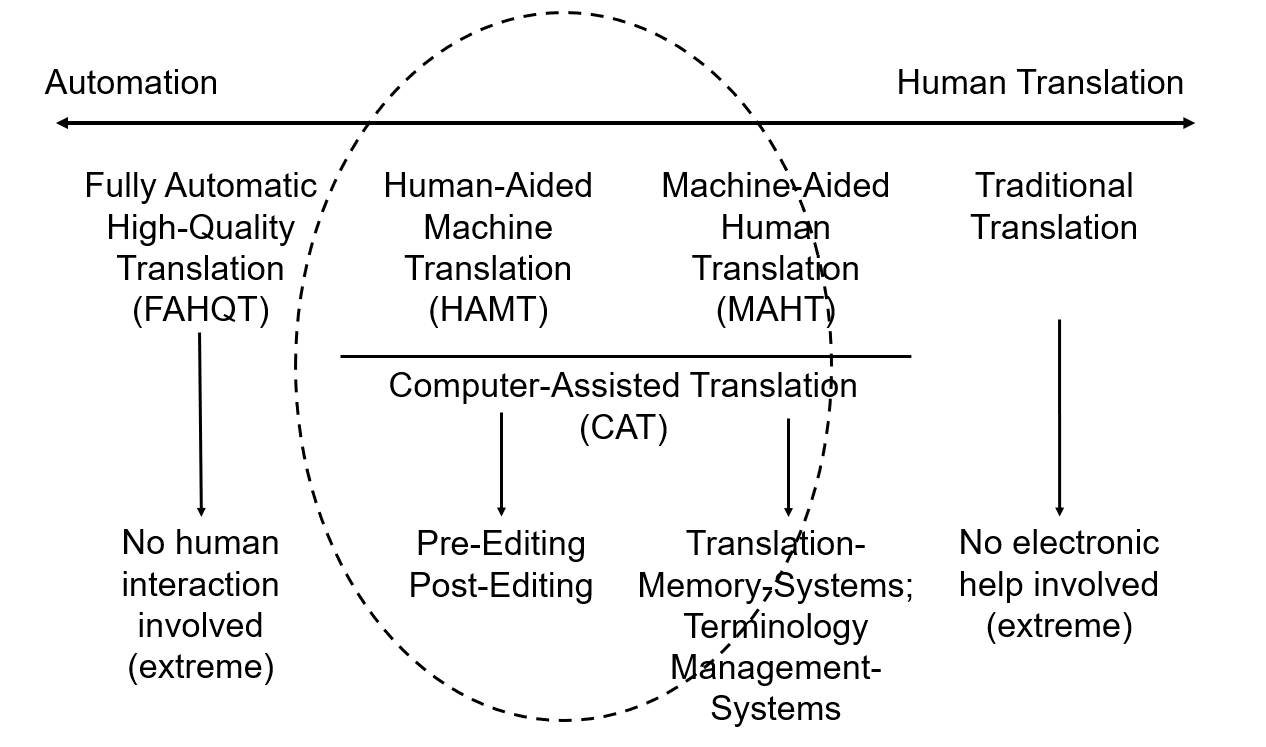
\includegraphics[height=0.45\textheight]{figures/Dimensions of HT and MT.png}
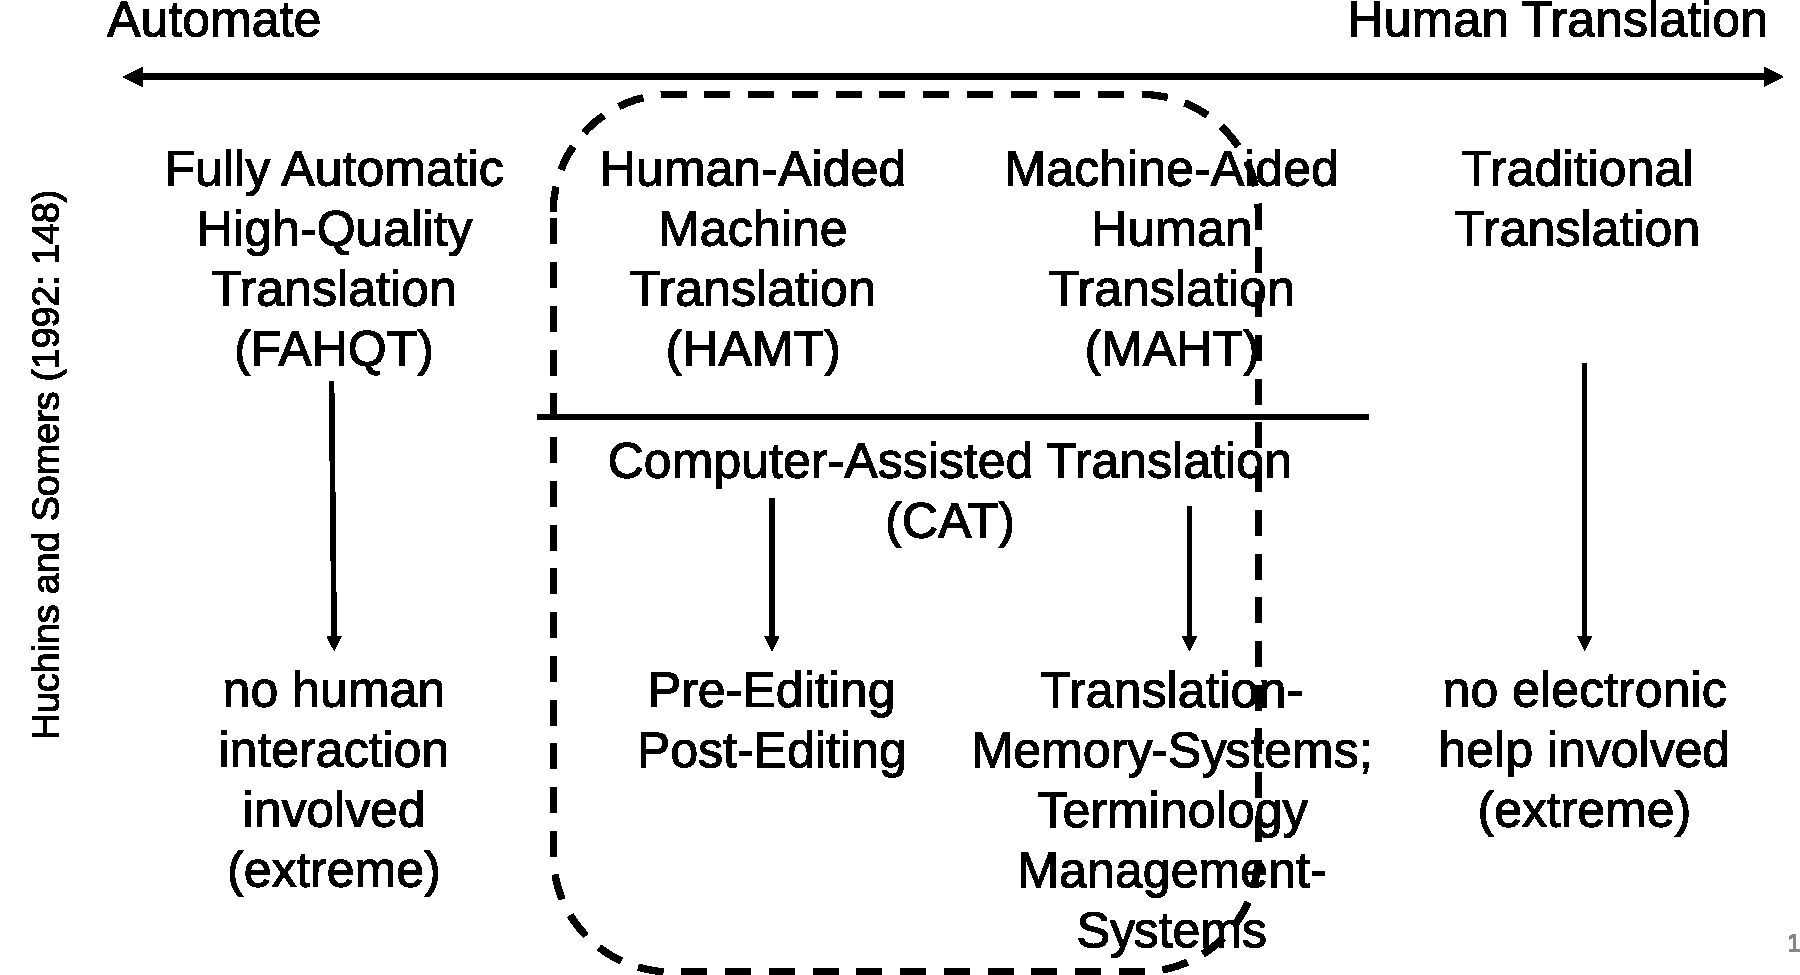
\includegraphics[width=\textwidth]{figures/Dimensions of HT and MT.pdf}
\caption{Dimensions of human and machine translation adapted from \citet[148]{hutchins1992introduction} }
\label{fig:key:2:1}
\end{figure}

As in many other disciplines, buzzwords such as ``digitalisation", ``artifical intelligence" or ``industry 4.0" have also become relevant in translation studies and practice in recent years. In fact, we have been moving towards the automatisation of translation for decades now. We can imagine the automatisation process of translation as a scale. At one end of the scale (in \figref{fig:key:2:1} on the right), we have human translation. The very end of the scale implies that no electronic aids would be involved. The translators would translate using pen and paper, printed dictionaries and the source text document would also be available as a printed version. At the other end of the scale, we find fully-automatic, high-quality machine translation (FAHQMT). So, the human translator would have no involvement in the translation process at all, except for providing the source text to the machine and receiving the target text. We might argue that both extremes are similarly unlikely. Maybe there are some scenarios where humans and machines do not interact in the translation process at all, but those are rather unlikely.\footnote{Of course, this again refers to professional translation practice. Some students still have to write their exams at universities with pen and paper -- the pros and cons of this procedure, however, will not be discussed here. Similarly, there have been scenarios for FAHQT for very restricted text types for decades. See e.g. the Météo system from Canada in \sectref{sec:3:1}.} At the moment, we are somewhere in between both extremes -- and, as mentioned earlier, we have been there for a while now. Since the 1990s, professional translators have been using CAT tools, a term which typically refers to translation memory systems, terminology management systems and project management systems (for a quick introduction, see e.g. \citealt{folaron2010translation}). 
However, the use of word processing programs or electronic/online dictionaries also counts as a step towards automatisation. When those tools are used, we speak of machine-aided human translation (MAHT). The human is still at the centre of the translation process, but is supported by the machine. One further step towards automatisation is what is called human-aided machine translation (HAMT). Here, MT systems are involved and the human ``solely" has to prepare the source text for the machine (pre-editing) and/or improve the MT output (post-editing). The latter is what we will focus on in this book (marked in a dotted line in \figref{fig:key:2:1}). What you have to keep in mind, though, is that MT output is still only a tool for the professional translator (if you do not agree now, you will probably agree after you have finished the book). The focus in pre- and post-editing is more on the machine and a certain amount of the work is performed by the machine. However, the professional translator is still responsible for transforming the MT output into a translation that matches the quality criteria defined for the target text.


%ich weiß nicht, wie ich die Zeile "of HT and MT.png of HT and MT.bb" rauskriege...

As \cite{allen_post-editing_2003} already pointed out, PE introduced a new perspective to translation studies, because translators never really had to deal with ``half-finished" texts before. In PE, the target text does not need to be produced from scratch. The translators already have an outline for the final product. Hence, PE and human translation can be considered different tasks. Further, machine-translated texts have different characteristics than human translations. Therefore, PE cannot be seen as another form of proof-reading either. While some mistakes, like spelling and typing errors, hardly ever occur in MT output, other mistakes, e.g. syntax or lexicon errors, would almost never occur in human translation. Accordingly, there are many interesting questions that must be answered to define the nature of PE. Here, we have only listed a few:
\begin{itemize}
    \item How much MT is acceptable?
    \item How much PE effort is necessary?
    \item How much time (and money) can be saved?
    \item What is the quality of the post-edited target text?
    \item What is the difference from human translation/proof-reading?
\end{itemize}
We will discuss all these questions in the following sections, providing you with a grounded understanding by the time you finish this book.

\bigskip

From a research point of view, post-editing “is a field in which the human translator and the machine meet – as well as the two disciplines Machine Translation and Translation Science” \citep[35]{culo_influence_2014}. Hence, it is very interesting for interdisciplinary research as well. 
Since this book is intended to be a rather practical guidebook, we do not want to go into detail concerning scientific research on post-editing. We just want to say a few words on the importance of research for this subject matter and where you can find relevant literature and databases with empirical PE data.

First of all, we want to clarify that there are some initial approaches to basic theoretical research concerning PE. One promising theory to describe PE phenomena seems to be the relevance-theoretical approach as cognitive and pragmatic aspects are connected. Post-editors are trained professionals who are able to bridge a communicative gap between languages by editing machine translation output situated in the target context. This task is based on well-founded decisions regarding the source text, the intended recipients, the target culture and the post-editing brief. On a cognitive level, relevance theory assumes that MT output should be edited with the least possible effort envisaging efficient and successful communication. \citet{alves2016investigating} discussed relevance-theoretical aspects for PE. The temporal and cognitive effort is ideally reduced during post-editing as translation options are suggested by the MT system, which the post-editor “solely” has to accept, reject or modify. Typically, guidelines are provided for each PE project to support the post-editors’ decision-making process. A rule that often occurs in PE guidelines is that as much of the raw MT output as possible should be retained to make the process fast and efficient. This also has the advantage for the client that the costs for the translation process decrease. On the other side, however, this also means that the recipients are expected to invest more cognitive effort when reading the target texts as the texts are not linguistically and/or stylistically perfect. \citet{carl2019outline} combined relevance theory and the noisy channel model to approach PE theoretically. They propose a “model in which [relevance theory] complements the ‘Noisy Translator Channel’ by adding constraints of causal interrelation between stimulus, context and interpretation, established by the principle of relevance.” \citep[60]{carl2019outline}


In addition to these theoretical considerations, there is a whole range of empirical studies comparing post-editing to translation-from-scratch, addressing the following research questions (of course, this is only a selection): 
\begin{itemize}
    \item How efficient is PE compared to human translation?
    \item Can cognitive effort while post-editing MT be measured?
    \item How good is the quality of post-edited texts? 
    \item Can MT errors be predicted and PE effort be estimated?
    \item Can PE effort be correlated to MT quality?
    \item Are some language pairs more suitable for MT and PE than others?
    \item Which text types, genres and modalities are particularly suitable for post-editing?
    \item Is there a difference in PE performance when comparing students and professionals?
\end{itemize}

From a methodological point of view, most studies rely on a multi-method approach combining eyetracking with keylogging data. In addition, questionnaires describe the metadata with respect to the participants, such as personal data as well as translation and language competence and experience. There is a widely established research database that includes PE and translation data for several language pairs and levels of expertise: the CRITT Translation Process Research Database (CRITT TPR-DB, \citealt{carl2016critt}). This database enables the triangulation of different kinds of data, which in turn sheds light on sequential and parallel cognitive processing activities, reading and writing processes, post-editing and research strategies. If you would like to learn more about the database, the studies and the resulting publications, please consult the following \href{https://sites.google.com/site/centretranslationinnovation/tpr-db}{website}\footnote{last accessed 12 April 2021}.

\newpage

\section*{Crossword puzzle -- chapter 2}

\begin{Puzzle}{12}{15}
|{} |[5]R 	|{} |{}  |{}     |{}  |{}     |{}  |{}    |{}  |{}    |{}   |.
|{} |[6]E   |M  |P |I    |R |I    |C |A   |L |{}    |{} |.
|{} |L   	|{} |{} |{}  |{} |{}    |{} |{}   |{} |{}    |{}   |.
|{} |[7]E   |Y 	|E  |T  |R  |A  |[3]C  |K    |I  |N     |G    |.
|{} |V   	|{} |{} |{} |{} |{} |A |{}   |{} |{}    |{}   |.
|{} |A   	|{} |{} |{} |[4]P |{} |T |{} |{}  |{}     |{}    |.
|{} |N    	|{} |{} |[8]C |R |I    |T |T   |{} |{}    |{}   |.
|{} |C   	|{} |{} |{} |E  |{}  |O  |{}    |{}  |{} |{}    |.
|{} |E   	|{} |{} |{} |E |{}   |O |{}   |{} |{}     |{}   |.
|{} |{}   	|{} |{} |{} |D |{} 	 |L  |{}    |{}  |{}     |{}    |.
|{} |{}   	|{} |{} |{} |I |{}   |S |{}   |{} |{}     |{}   |.
|[2]E  |F   |F  |O |R  |T |{}    |{} |{}   |{} |{}    |{}   |.
|{} |{}   |{}   |{} |{}|I |{}    |{} |{}   |{} |{}    |{}   |.
|{} |{}   |[1]T |R |A    |N |S    |L |A   |T |O    |R   |.
|{} |{}   |{}   |{}|{}   |G |{}    |{} |{}   |{} |{}    |{}   |.
\end{Puzzle}

\begin{PuzzleClues}{\textbf{Across}}
\Clue{1}{TRANSLATOR}{Who should be the post-editor? A professional ...}
\Clue{2}{EFFORT}{Specific guidelines and quality criteria define how much ... a post-editor has to put into the post-editing job.}
\Clue{6}{EMPIRICAL}{What kind of studies exist about post-editing aside from theoretical considerations?}
\Clue{7}{EYETRACKING}{What kind of methodology is often used in cognitive translation studies in addition to keylogging?}
\Clue{8}{CRITT}{What is the name of the Translation Process Research Database?}
\end{PuzzleClues}

\begin{PuzzleClues}{\textbf{Down}}
\Clue{3}{CATTOOLS}{What is the term that refers to translation memory systems, terminology management systems and project management systems?}
\Clue{4}{PREEDITING}{What do we call the preparation of the source text for machine translation?}
\Clue{5}{RELEVANCE}{According to which theory would we assume that MT output should be edited with the least possible effort to achieve the most efficient and successful communication?}
\end{PuzzleClues}
 
\chapter{MT history -- how has machine translation developed?}\label{sec:3}

    \objectives{
        You will learn...
        \begin{itemize}
            \item how MT developed in the last decades,  
            \item how the different MT systems generate their translation,
            \item how suitable the different MT architectures are with respect to post-editing. 
        \end{itemize}
        }

\vspace{\baselineskip}

You might get the impression that MT is a rather new invention because it became increasingly visible with the rise of statistical and especially neural MT engines. However, the first ideas about automating language and translation date back centuries. In order to understand which approaches are suitable for post-editing and under which conditions, it is important to learn something about the commonalities and differences of the MT architectures and how they developed over time. 

This section will shed light on the historical development of MT in \sectref{sec:3:1} and will introduce the basic MT approaches and discuss their suitability with respect to post-editing in \sectref{sec:3:2}.

\section{Historical development of MT}\label{sec:3:1}

The following table (\ref{long}) will show you the most important historical milestones starting from the 1930s with the first events that initiated the actual development of the first systems. The notion of automating translation processes is much older, however it was only theoretical then.

If you want to learn more about the historical development of MT, we recommend reading, for example, \citet{hutchins2000early}, \citet{hutchins2007machine}, and/or \citet{schwartz2018history}.

 \begin{longtable}[c]{ |>{\raggedright}p{2.8cm}||p{8.5cm}|  }
 \caption{History of MT.\label{long}}\\\hline
 \multicolumn{2}{| c |}{History of MT}\\\hline
 Event & Description\\\hline
 \endfirsthead
 
 \hline
 \multicolumn{2}{|c|}{History of MT}\\ \hline
 Event & Description\\ \hline
 \endhead
 
 \hline
 \endfoot
 
 \hline
 \multicolumn{2}{| c |}{Future}\\ \hline\hline
 \endlastfoot
 
 1933 - 
 
 First patents for ``Translating Machines" & The French-Armenian Georges Artsrouni and the Russian Petr Troyanskii independently proposed patents for ``translating machines" as early as 1933. Troyanskii proposed not only a method for an automatic bilingual dictionary on paper tape, but also a scheme for coding interlingual grammatical roles (based on Esperanto) and an outline of how analysis and synthesis might work. However, Troyanskii’s ideas were unknown to the community until the end of the 1950s.\\ \hline
 1949 - 
 
 Weaver Memorandum & A memorandum titled ``Translation" by Warren Weaver in July 1949 introduced the idea of MT to the general public. It is often considered the starting point of research on MT.\\ \hline
 1952 - 
 
 First MT conference & The first full-time researcher in MT was appointed at the Massachusetts Institute of Technology (MIT) in 1951, namely Yehoshua Bar-Hillel. He believed that fully-automatic, high-quality translation (FAHQT) could be possible. In 1952, the first conference on MT was held at MIT and covered topics such as pre-editing and post-editing, controlled language, domain restrictions, syntactic analysis as well as computer hardware, programming and funding.\\ \hline
 1954 - 
 
 Georgetown–IBM Experiment & During the Cold War, the first official MT projects were launched for the US military and also in the Soviet Union. Those projects focused on MT between Russian and English. They produced rather poor quality but were still popular for political and military reasons. Thus, most US research was for Russian-English translation, and most Soviet research was on English-Russian systems. The focus was on purely informative translation purposes without PE or any involvement of third-party translators or interpreters. 
 
 At Georgetown University, Leon Dostert collaborated with IBM on a project known as the Georgetown–IBM experiment which resulted in the first public demonstration of an MT system in January 1954. The project involved the fully automatic translation of more than sixty sentences from Russian into English. The experiment, which was conducted with well-chosen sentences, launched the first MT hype. This stimulated large-scale funding of MT research in the USA and inspired the initiation of MT projects elsewhere in the world, notably in the USSR.\\ \hline
 1961 - 
 
 Machine Translation Research in Texas & The Linguistic Research Center (LRC) at the University of Texas concentrated on basic syntactic research of English and German. Efforts were made to devise reversible grammars to achieve bidirectional translation within an essentially ``syntactic transfer" approach. This laid the foundations for the later successful development of the METAL system which started in 1979 in cooperation with Siemens AG.\\ \hline
 1966 - 
 
 ALPAC Report announces FAHQT impossible & In November 1966, the Automatic Language Processing Advisory Committee (ALPAC) issued a report to the Pentagon which brought the substantial funding of MT research in the United States to an end for about twenty years. The clear message of the ALPAC Report to the general public and the rest of the scientific community was that there is basically no hope for MT. The title of the report was ``Languages and machines: computers in translation and linguistics". Supposedly, it dealt not just with MT but also with computational linguistics. However, in practice, most funded NLP research was devoted to developing MT at the time.\\ \hline
 1968 - 
 
 The Beginnings of Systran & Engineering companies continued less visible research on MT. IBM developed the first commercial statistical machine translation system (SMT) Systran in 1968. Systran is one of the oldest MT companies and was founded by Peter Tome.\\ \hline
 1970-1978 - 
 
 Météo & In 1970, research began on a syntactic transfer system for English-French translation at Montreal. The TAUM project (Traduction Automatique de l'Université de Montréal) had two major achievements: the Q-system formalism, a computational metalanguage for manipulating linguistic strings and trees and the foundation of the Prolog programming language widely used in natural language processing; and secondly, the Météo system (1978) for translating English weather forecasts into French.\\ \hline
 1972-1986 - 
 
 SUSY & Researchers at Saarbrücken University developed SUSY (Saarbrücker Übersetzungssystem), a highly-modular multilingual transfer MT system.\\ \hline
 1976 - 
 
 EC and Systran & The European Commission first introduces Systran for in-house purposes.\\ \hline
 1978-1992 - 
 
 The EUROTRA project & The EUROTRA project was founded by the European Commission with the aim of developing a state-of-the-art MT system for the then seven, later nine, official languages of the European Community. In 1978, research on different MT projects began, e.g. research leading to the ARIANE system at Grenoble University (Russian-French-English-German), the LOGOS system (USA; now OpenLogos for German-English), and the GRADE system within the Mu project at Kyoto University (Japanese-English).\\ \hline
 1985 - 
 
 Prolog & In 1985, the Japanese government started the 5th Generation Project and developed the Prolog programming language for commercial MT which led to the development of LMT (Logic programming MT).\\ \hline
 1989 - 
 
 METAL System & Already in the 1970s, Siemens started working on a transfer approach for a machine translation system together with the LRC (Linguistic Research Centre) in Texas. Originally titled the Linguistics Research System (LRS), it was later renamed METAL (Mechanical Translation and Analysis of Languages) and finally became commercially available in 1989.\\ \hline
 1992 - 
 
 Automatic Evaluation of MT & The development of MT evaluation metrics started simultaneously with the development of statistical MT systems. Initial evaluations were carried out by human assessors according to FEMTI (Framework for the Evaluation of Machine Translation in ISLE). In 1992/1994, DARPA -- a research agency of the United States military -- investigated unedited output of MT systems, comparing automatic measures and human judgments of adequacy, fluency, informativeness.\\ \hline
 1993 - 
 
 Translation Memory Systems & The first commercial translation memory system, launched in the 1990s, was named TRADOS (TRAnslation and DOcumentation Software) and used aligned bilingual corpora. Trados was established in Stuttgart, Germany by Jochen Hummel and Iko Knyphausen in 1984. \\ \hline
 1997 - 
 
 First free online MT & After Systran started offering its service of online machine translations of entire webpages, the first free online machine translation was launched in December 1997 with Babel Fish on Alta Vista (later Yahoo) which was free for all Internet users but was discontinued in 2008.\\ \hline
 2000-2001 - 
 
 Crash of dotcom companies & After the crash of the dotcom companies in 2000, the number of MT software companies decreased to 10-20 active companies and universities that were working on MT. They made up only 1\% of revenue on the translation market despite the growing demand for MT applications. The still growing number of digitally available texts due to globalisation requires more translations with all sorts of language combinations even today.\\ \hline
 2001-2005 - 
 
 BLEU & In 2001, the BLEU score (Bilingual Evaluation Understudy) was developed which consists of statistical measures of similarity of SMT output and human (reference) translations. Other automatic evaluation scores include the NIST metrics by the National Institute of Standards and Technology and METEOR (Carnegie Mellon) in 2005.\\ \hline
 2002 - 
 
 Language Weaver & Language Weaver is the first company to commercialise a statistical approach to automatic language translation and natural language processing, which was founded by Kevin Knight and Daniel Marcu in 2002.\\ \hline
 2003-2004 - 
 
 Expansion of EU and growing demands & With the expansion of the EU, the number of official languages increased from 11 to 20 languages. At peak times, the European Union produced more than 1.4 million pages of text per month. Since then, about 380 language combinations are possible for translation at the EU, which can no longer only be covered by human translators.\\ \hline
 Since 2004 - 
 
 Open Source toolkits for MT & With the growing demand for language pairs numerous open source toolkits for MT systems appeared. Examples are: GIZA ++ (alignment tool for SMT); Moses (a platform for building SMT systems); Joshua (a decoder for syntax-based, hierarchical SMT); Apertium (a platform for building rule-based MT); META-SHARE (database for EU projects)\\ \hline
 2006 - 
 
 Google Translate SMT and Euromatrix & On 28 April 2006, Google Translate went online with a statistical MT system. The first system used transcripts from the UN and the European Parliament to gather enough training material. Further, the system used English as a transfer language. Later, Google expanded to further language pairs and applied a hybrid method. Around the same time, the Euromatrix project was founded with the aim of providing MT systems for all EU languages (over 500 language pairs), which involved a different research partner.\\ \hline
 2010 - 
 
 SDL Acquires Language Weaver & In July 2010, the leading language services company SDL acquired Language Weaver/ BeGlobal Statistical Machine Translation and the MT system became SDL Language Weaver.\\ \hline
 2016 - 
 
 Google introduces NMT & In 2016, Google Translate was one of the first to introduce neural machine translation (NMT). In November 2016, software engineer Harold Gilchrist, leader of the Google research team developing the Google Neural Machine Translation system (GNMT) to increase fluency and accuracy in Google Translate, announced the switch from SMT to GNMT.\\ \hline
 2016 - 
 
 SDL Adaptive MT & SDL introduces Adaptive MT for SDL Trados Studio 2017 - a self-learning machine translation engine.\\ \hline
 2017 - 
 
 DeepL is introduced & DeepL is another NMT system that was introduced by the online dictionary and corpora provider Linguee.\\ 
\end{longtable}




\section{MT architectures}\label{sec:3:2}

As you have seen above, different approaches have been developed to automatise the translation process. Here, we will discuss the pros and cons for rule-based, statistical and neural MT and their usability for PE workflows. 

\subsection{Rule-based machine translation (RBMT)}\label{sec:3:2:1}

Rule-based approaches were the catalyst for the development of MT. Generally, these systems attempt to define the individual characteristics of the source language and how these need to be converted into the target languages. \citet[31]{chesterman1997memes} mentions that he sees this early form of MT as “the Linguistic meme of translation theory”, because it assumes that languages can solely be expressed through rules, which, accordingly, must also be representable in algorithms. Different rule-based approaches had been developed over the years to generate MT:

 \begin{itemize}
    \item Direct MT: This type of MT is constructed specifically for one language pair and usually one translation direction. Essentially, the words of the source text are morphologically analysed and then looked up in a dictionary, which means that ideally all morphology rules are defined, so that the dictionary only has to contain the stems of the words. In the next steps, the words of the source language are replaced by the words in the target language and all morphological changes required by the target language are applied.
    \item Transfer-based MT: The transfer-based approach constructs a syntactic representation of the source text (often in a tree structure) that is free of ambiguities, etc. Next, this representation is generated for the target language with the help of a grammar that contains the bilingual transfer rules. The target text can be produced now. It is possible to use these systems in both language directions, but this is rarely done in practice, because the transfer rules often cannot be applied in both directions.
    \item Interlingua-based MT: For this approach, a so-called Interlingua needs to be created. This Interlingua represents meaning in an abstract form, which can theoretically be achieved by either a natural or an artificial language or a language-independent representation. The basic principle of this approach is that the source text is translated into the Interlingua and then the Interlingua into the target language. This approach is suitable for multilingual systems.
\end{itemize}

Please note that this is only a brief introduction to the main concepts of these approaches. For overviews on rule-based approaches see \citet{hutchins1992introduction} or \citet{wilks2008machine}. You can find a visualisation of the different rule-based approaches in \figref{fig:key:4:1}. This pyramid was introduced by \citet{vauquois1968survey} and shows the different steps that lie between source text and target text generation.

\begin{figure} 
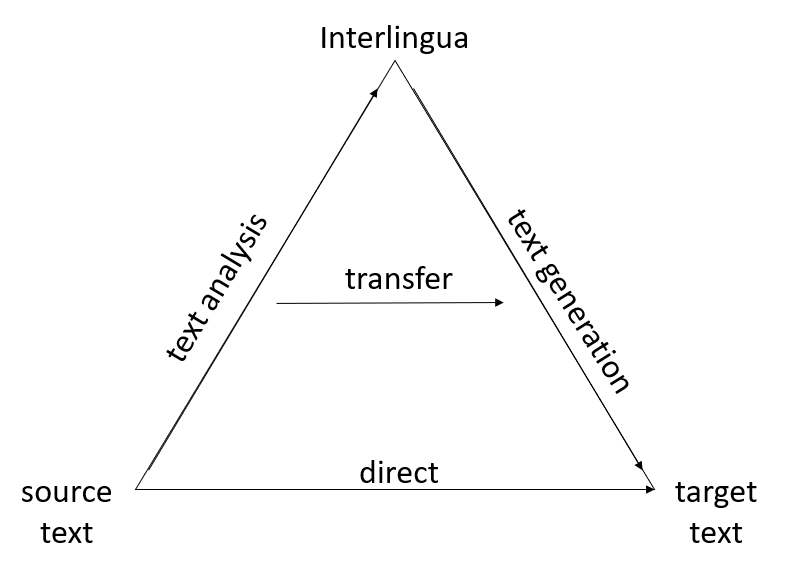
\includegraphics[height=0.4\textheight]{figures/Vaquoise triangle.PNG}
\caption{Vauquois pyramid \citep{vauquois1968survey}}
\label{fig:key:4:1}
\end{figure}


\largerpage[1.5]
Concerning PE, this approach seems especially suitable for the translation of texts adhering to a controlled language. Controlled languages are defined by a set of rules, which can theoretically be directly implemented into rule-based systems. The main disadvantage of these approaches is, however, that it takes a lot of effort to develop the systems, because the better and more comprehensive the intended system, the more rules have to be defined. If morphology, grammar, and syntax are only defined superficially, the source text might be generated incorrectly, which leads to (severe) mistakes in the target language. Further, the rules have to be defined from scratch for every language involved or sometimes even for every language direction, depending on the MT approach. 

Today, rule-based approaches are outdated and can usually only be found in hybrid systems or in very old, established systems. For example, the Pan American Health Organization (PAHO) still uses a rule-based system, because they already established their MT system in the 1980s and traditionally work with only three languages.\footnote{Find out more on the \href{https://www.paho.org/hq/index.php?option=com_content&view=article&id=14762:machine-translation-at-the-pan-american-health-organization&Itemid=1896&lang=en}{PAHO's webpage on their MT system PAHOMTS}, last accessed 27 April 2021.}\clearpage


More promising are data-based approaches, which render the human programming of linguistic rules for MT unnecessary. Data-based MT relies on mono- and multilingual corpus data. The following sections will give an overview of the most prominent data-based MT architectures: statistical machine translation (SMT) and neural machine translation (NMT).



\subsection{Statistical machine translation (SMT)}\label{sec:3:2:2}

SMT had been the state of the art for decades. The basic idea of this approach is to generate a translation from a parallel training corpus by calculating the most likely equivalent of a source word/phrase/sentence in the target language. Statistical translation models are generated and trained on corpus data. Both mono- and bilingual corpora are used to capture the typical linguistic structures of the languages involved – the monolingual corpora generate the target language model and the bilingual parallel corpora generate the translation model. In addition, SMT uses so-called n-grams – sequences of aligned words (usually n≤7) assigned with probabilities, which represent how likely the word sequences occur in the training corpus. Further, additional information can be extracted during the training phase, e.g. models of relative sentence length. The training of SMT systems can be realised relatively quickly if aligned parallel corpora are available. Training means in this context that the source text is analysed. Decoding, on the other hand, means in this context that the target text is generated. In between, there is the tuning phase, where the system tries to find the best values for the respective sentences or n-grams. Two models are commonly differentiated to calculate the most likely translation: the noisy channel model and the log-linear model. We do not want to go into detail here, please refer to \citet{hearne2011statistical} for further information.

In addition to the translation and language models, other features that contain linguistic information can be implemented to help calculate the most likely translation. These include a phrase table for each language direction, lexical translation probabilities, a model for phrase reordering, or a word or phrase penalty that controls the length of the target sentence. All these features help to calculate the most likely translation and select it among other translation candidates. Each feature obtains a value that represents its weight in the algorithm.

A final training task involves the evaluation of the system’s performance and the adaptation of the values that are given to the single features. One widely adopted technique to estimate the system is the so called MERT technique, which is short for Minimum Error Rate Training (see also \citealt{och2003minimum}). The MERT technique usually includes the BLEU metric. To keep it simple, this is an automatically calculated value that evaluates the quality of an MT system by comparing the translation output of the system to a reference translation.

An advantage of post-editing SMT texts is that the errors to be corrected are quite predictable. SMT systems always produce the same errors as long as they are not trained with new or extended training corpora. The code of the system is transparent and the calculation of translation probabilities straightforward. For a given language direction, typical errors can be identified, i.e. that the post-editor can systematically train error spotting and correction (\citealt{culo_influence_2014}, \citealt{nitzke2019problem}). 

Recent developments involving SMT have attempted to unite different approaches – usually rule-based and statistical – in hybrid systems so that the advantages of each approach can be combined. Systems with deep integration construct a whole new system that combines the advantages of the two approaches. Shallow integration systems, on the other hand, unite two or more existing systems into one new system.

\subsection{Neural machine translation (NMT)}\label{sec:3:2:3}

The latest approach to MT is the use of neural networks and can also be applied to parallel training corpora. NMT systems build large neural networks for translation, while statistical MT systems are composed of many small subcomponents. NMT systems use deep-learning approaches and learn automatically from the training data. 

At least three basic layers are involved in neural machine translation: the input layer, the output layer and at least one hidden layer in between. In the input layer, the source text is processed and in the output layer, the target text is created. The hidden layers are the processing steps. The model can work in a more fine-grained way and more complex tasks can be tackled when more hidden layers are included in a system. During training, mathematical representations and weights are assigned to the source and target segments in the training data. The training is comparably time-consuming as the system runs through the training data several times to adjust this structure. Further, no specific rules can be added manually, as the system develops the structure of the hidden layers automatically. Hence, only input and output layers are known, but the rest is more or less a blackbox (see \citealt{koehn2017neural} for detailed information), although tools and methods have been developed to interpret the decisions within a system (e.g. \citealt{vig2019bertviz})

Two approaches are common in neural machine translation: transformer and recurrent encoder-decoder models. In the encoding phase, the meaning of the source text is encoded into a vector with a fixed length. Transformer and recurrent systems differ in the way they encode the source text. In the decoder phase, the target segment is produced word for word. During the production, the system considers the surrounding words as context. One disadvantage of this system is that it has difficulties with long sentences. To overcome these problems, so called alignment models are implemented. These are often also called attention models. To improve the translation output, an additional layer is put between the input and the hidden layer. This additional layer embeds words, which means that the system is capable of considering context. This means that all content words are assigned to a representation. Words that are close content-wise are represented closely. Hence, similar words are clustered and are translated in similar manners. If you want to learn more on the architecture of NMT systems, read the comprehensible introduction by \citet{perez-ortiz_how_nodate}.

As the current NMT systems for interlingual translation currently outperform all other systems in many cases (\citealt{bentivogli2018neural}; \citealt{toral2017multifaceted}), not only redundant and highly standardised text types are in the focus of attention (as is the case in technical documentation, software localisation etc.), but also creative text types such as literary translation \citep{toral2018post} or subtitling \citep{tardel2020effort}. It might also be very interesting to test NMT for intralingual translation by translating Standard Language into Easy Language (as can be found in approaches to automatic text simplification, see \citealt{specia2010translating}). For example, it seems plausible that the neural networks might be able to represent the rules for translating standard German into Easy German during the training phase. For this purpose, a parallel corpus of standard German source texts and Easy German target texts will be necessary (e.g. \citealt{klaper2013building}). An NMT system which differentiates between different scales of complexity and difficulty (Easy Language -- Plain Language -- Standard Language -- Specialised Language) would revolutionise the whole area of accessible communication.

With respect to PE, one of the advantages of NMT is that the machine-trans\-lated output seems to be (much) better compared to other system architectures, at least when it comes to fluency. However, we can only get good results in the MT output if we have enough training material to feed the system. If we do not have enough training material, we get poor quality. This is often problematic for smaller languages and rare language combinations as they are often underrepresented and poor in resources. Further, as with all data-driven MT systems, the output can only be as good as the training data. Hence, if we train a system with poor quality translations, we get poor output. The same applies for domain specific translations. If the system is not well-trained on the specific domain, the output is poor as well. In total, the system is much more vulnerable to noisy data. Newest developments, however, allow the combination of NMT and the training of specific terminology, which tackles the domain problem (e.g. \citealt{michon2020integrating}). Another advantage is that NMT systems contain one compact system that does not have several components. However, training takes much longer than it takes for SMT and it also needs more computer processing capacities.

Finally, we want to point out that the generally better NMT output quality leaves us with the following paradox: the better the NMT translations are, the more difficult the error spotting is since the NMT output appears to be more fluent and less error-prone. This makes, on the one hand, the PE process even more demanding and leads to more cognitive effort for the post-editor. On the other hand, due to the absence of ``real" errors, the post-editors tend to correct more style errors, which in turn leads to over-editing (for details see \citealt{vardaro2019translation}). Hence, post-editors need a lot of training and awareness for the error types to be able to correct the texts efficiently.

\section*{Crossword puzzle -- chapter 3}

\begin{Puzzle}{15}{16}
|{}	|{}	|{}	|{}	|{}	|{}	|{}	|{}	|[6]W	|{}	|{}	|[8]S	|{} |{} |{} |.
|{}	|{}	|{}	|{}	|{}	|{}	|{}	|{}	|E	|{}	|{}	|T	|{} |{} |{} |.
|{}	|{}	|{}	|[3]R	|U	|S	|S	|I	|A	|N	|{}	|A	|{} |{} |{} |.
|{}	|{}	|{}	|{}	|{}	|{}	|{}	|{}	|T	|{}	|{}	|T	|{} |{} |{} |.
|[7]B	|A	|B	|E	|L	|F	|I	|S	|H	|{}	|{}	|I	|{} |{} |{} |.
|{}	|{}	|{}	|{}	|{}	|{}	|{}	|{}	|E	|{}	|{}	|S	|{} |{} |[9]I |.
|{}	|{}	|{}	|{}	|{}	|[2]G	|E	|O	|R	|G	|E	|T	|O |W |N |.
|{}	|{}	|{}	|{}	|{}	|{}	|{}	|{}	|F	|{}	|{}	|I	|{} |{} |T |.
|{}	|{}	|{}	|{}	|[10]N	|{}	|{}	|{}	|O	|{}	|{}	|S	|{} |{} |E |.
|{}	|{}	|{}	|[1]W	|E	|A	|V	|E	|R	|{}	|{}	|T	|{} |{} |R |.
|{}	|{}	|{}	|{}	|U	|{}	|{}	|{}	|E	|{}	|{}	|I	|{} |{} |L |.
|[5]S	|Y	|S	|T	|R	|A	|N	|{}	|C	|{}	|{}	|C	|{} |{} |I |.
|{}	|{}	|{}	|{}	|A	|{}	|{}	|{}	|[4]A	|L	|P	|A	|C |{} |N |.
|{}	|{}	|{}	|{}	|L	|{}	|{}	|{}	|S	|{}	|{}	|L	|{} |{} |G |.
|{}	|{}	|{}	|{}	|{}	|{}	|{}	|{}	|T	|{}	|{}	|{}	|{} |{} |U |.
|{}	|{}	|{}	|{}	|{}	|{}	|{}	|{}	|S	|{}	|{}	|{}	|{} |{} |A |.
\end{Puzzle}

\begin{PuzzleClues}{\textbf{Across}}
\Clue{1}{WEAVER}{Who wrote the memorandum titled ``Translation" published in 1949?}
\Clue{2}{GEORGETOWN}{Which university hosted the first public demonstration of an MT system in January 1954?}
\Clue{3}{RUSSIAN}{Which languages were involved in the first public demonstration of an MT system in January 1954? English and ...}
\Clue{4}{ALPAC}{What was the name (abbreviation) of the report that ended funding of MT research in the United States for about twenty years?}
\Clue{5}{SYSTRAN}{What is the name of one of the oldest MT companies that was founded by Peter Tome?}
\Clue{7}{BABELFISH}{What was the name of the first free online machine translation that was launched in December 1997?}
\end{PuzzleClues}

\begin{PuzzleClues}{\textbf{Down}}
\Clue{6}{WEATHERFORECASTS}{What was translated by the Météo system?}
\Clue{8}{STATISTICAL}{With what kind of approach did Google launch their first online MT system?}
\Clue{9}{INTERLINGUA}{What is the name of a language that represents meaning in an abstract form?}
\Clue{10}{NEURAL}{What is the state-of-the-art MT approach? ... MT}
\end{PuzzleClues}
 
\chapter{Post-editing guidelines -- how to post-edit?}\label{sec:4}


\objectives{
        You will learn...
        \begin{itemize}
            \item about different guidelines, especially light and full PE,
            \item about monolingual PE and the associated problems,
            \item what is included in the PE Norm,
            \item how to adhere to different guidelines.
        \end{itemize}
        }

\vspace{\baselineskip}

Every translation and thus also every PE project has different requirements. Especially in PE, the required target text quality might vary a lot, depending on various factors like reader, distribution, or duration of use. Hence, the effort invested in the PE process might differ and how much effort should be invested while post-editing a text has to be defined in advance. 

\section{Considerations on PE guidelines}\label{sec:4:1}

You might wonder why we need guidelines for PE. PE is not per se intended to generate perfect, high quality texts. The main goal is to save time and money. Therefore, it is very important to define the final quality criteria and editing needs in advance. You have to ask yourself different questions to judge the required target text quality and thus the PE effort that needs to be invested. As these decisions are usually not made by the post-editors themselves, we will discuss the decision making process later in \sectref{sec:8}. For now, we have to keep in mind that we need PE guidelines to achieve the defined target text quality, which should ideally be communicated with the post-editing job. In addition, guidelines help us to make the target text as consistent as possible even if different post-editors work on the same text -- similar to the processes in technical documentation or other domain-specific translations. 

In general, we differentiate between light vs. full PE. This differentiation is quite superficial for real PE projects as discussed in \citet{nunziatini2020machine}. The guidelines might differ a lot from project to project and every PE project might focus on different quality aspects, e.g. using the correct, pre-defined terminology might be far more important in technical documentation than in post-editing a newspaper article. However, the differentiation between light and full PE is well-established and will give you an impression of the continuum in which we are working.

The guidelines we want to introduce to you were established by TAUS (Translation Automation User Society).\footnote{Find the guidelines and further recommendations on their \href{https://www.taus.net/academy/best-practices/postedit-best-practices/machine-translation-post-editing-guidelines}{webpage}, last accessed on 28 April 2021.} The society was established in 2005. It is an independent organisation that is concerned with automation and innovation in translation. 

\subsection{Light PE}\label{sec:4:1:1}

The first set of guidelines we want to talk about are what TAUS calls the guidelines for achieving “good enough” quality.\footnote{See also the discussions under the buzzword "fit-for-purpose translation", e.g. \citet{bowker2019}.} This equals what is generally considered light PE.

The criteria for “good enough” are defined by TAUS as follows: 

\begin{itemize}
    \item comprehensible: the contents of the text should be comprehensible
    \item accurate: the meaning of the source text should be preserved
    \item but stylistic quality plays a minor role
\end{itemize} 

This means that the text may appear unidiomatic and unnatural as it is generated by a computer. The grammar and syntax can be incorrect as long as the meaning is comprehensible. Concerning the guidelines for light post-editing, TAUS puts it this way: 

\begin{itemize}
    \item Aim for semantically correct translation. 
    \item Ensure that no information has been accidentally added or omitted.
    \item Edit any offensive, inappropriate or culturally unacceptable content.
    \item Use as much of the raw MT output as possible.
    \item Basic rules regarding spelling apply.
    \item No need to implement corrections that are of a stylistic nature only.
    \item No need to restructure sentences solely to improve the natural flow of the text.
\end{itemize}

The greatest challenge in light PE for most professional translators is leaving incorrect grammar and syntax unedited as we are usually used to creating high-quality translations. Keep in mind that you will not be paid for those corrections and try to remind yourself that for this job high quality is not needed. Light PE requires training and it will become easier to adhere to the guidelines after a while.

\subsection{Full PE}\label{sec:4:1:2}

Another set of guidelines are the guidelines for achieving quality that is similar or equal to human translation, often called full post-editing.
Besides being comprehensible and accurate (see above), stylistic quality is also important for full PE. However, it may still not be as good as it would be when translated from scratch. Syntax, grammar and punctuation need to be correct.
Concerning the guidelines for full post-editing, TAUS puts it this way: 

\begin{itemize}
    \item Aim for grammatically, syntactically and semantically correct translation.
    \item Ensure that key terminology is correctly translated and that untranslated terms belong to the client’s list of “Do Not Translate” terms.
    \item Ensure that no information has been accidentally added or omitted.
    \item Edit any offensive, inappropriate or culturally unacceptable content.
    \item Use as much of the raw MT output as possible.
    \item Basic rules regarding spelling, punctuation and hyphenation apply.
    \item Ensure that formatting is correct.
\end{itemize}

Full PE is more in line with the quality standards most professional translators are used to. However, it is still important to remember to use as much of the raw MT output as possible and to not get too lost in the fine-tuning.

\subsection{Monolingual PE}\label{sec:4:1:3}

Especially when talking to laypersons, the argument might come up that a post-editor only needs to be fluent in the target language, because the translation was created by the machine and the fine-tuning of the MT output takes place in the target text. However, think about whether you as a professional translator would be willing to revise a translation for which you do not know the source language or for which you do not have access to the source text. You would probably be reluctant to do so, because you know that many mistakes cannot be identified without the source text, especially content mistakes. And, as you can probably guess, this is also true for post-editing MT output -- maybe even more so.

Bilingual PE involves the comparison of source and target text. This means that the post-editor has to check the quality of the translation but he/she also has to assess whether the adequate meaning of the source text has been transferred by the MT system. In contrast, monolingual PE (MPE) suggests that the quality control of the translation can be carried out without taking the source text into account. The professional translation market and research on PE in translation studies hardly discuss MPE, but you should be aware that the option of MPE might come up when negotiating with clients. To have some arguments prepared, we want to discuss the topic briefly and present some findings of research on monolingual PE.

\citet{mitchell2013community} showed in their study that monolingually post-edited sentences are most often rated as an improvement to the pure MT output. However, there are also a number of incidents where the monolingual PE processes even negatively affected the final quality. This shows that monolingual PE mostly has a positive or neutral effect on the MT output, but it does not say whether the final product was good or even acceptable -- it was merely better than the pure MT output.

In her study, \citet{nitzke2016monolingual} compared the translation and PE products of 24 participants (twelve professionals, twelve students) for six texts that were translated/ post-edited from English to German. She found that ``superficial" mistakes like grammar, spelling, punctuation, etc. occurred similarly often in the final target texts for all three tasks (translation, bilingual PE, monolingual PE). However, content mistakes could be found much more frequently in the monolingually post-edited final texts than when the texts were translated from scratch or bilingually post-edited. However, we have to keep in mind that both studies used MT output of statistical MT systems.

When we talk about NMT, the picture is the same but different. Studies (e.g. \citealt{burchardt2017linguistic} or \citealt{macketanz2017machine}) showed that NMT generated translations still contain many errors, although it might seem that the quality of the MT output has improved for some language pairs as the output can be read more fluently. However, we assume that it might even become more difficult to find certain error types, especially content errors, even in bilingual PE, because the MT output is fluent and seems to be correct. Hence, the content mistakes are, in a way, more hidden.

Even though there might be some scenarios where monolingual PE may be sufficient or better than no PE at all (similar to how proof-reading a target text instead of revising it against its source text might be better than no quality assessment at all), we discourage you from engaging in monolingual PE in professional PE settings as some mistakes in the MT output cannot be found without consultation of the source text. Since monolingual PE neglects the assessment of the equivalence relations between source and target text, the adequacy of the meaning of the MT output cannot be evaluated at all. This therefore means that it is not possible to evaluate whether the output is accurate, i.e. whether the meaning of source and target text is identical. This is why we strongly recommend refusing jobs involving solely monolingual PE. The adherence to given standards (\sectref{sec:4}) is not possible at all for this kind of task and questions concerning risk assessment and liability (\sectref{sec:7}) cannot be addressed at all. 

\section{ISO 18587 -- the post editing standard}\label{sec:4:2}

In addition to the general guidelines, there is also an ISO standard addressing professional PE workflows. The PE standard ISO 18587 is called “Translation services — Post-editing of machine translation output — Requirements.” After having introduced the differences between light and full PE, we will now focus on this international standard and its requirements. We refer to the first edition which was published in April 2017.

The standard first discusses the reasons and advantages of post-editing machine translation: Translation costs can be decreased, the launch of products or the flow of information can be accelerated, translation productivity as well as the turn-around times can be improved, and translation service providers can remain competitive in a globalised world. Additionally, MT gives clients the possibility to translate material that could otherwise not be translated at all.

\begin{quote}
“However, there is no MT system with an output which can be qualified as equal to the output of human translation and, therefore, the final quality of the translation output still depends on human translators and, for this purpose, their competence in post-editing.” (DIN ISO \citealt[Introduction]{din_iso_18587_ubersetzungsdienstleistungen_2018})  \end{quote}

This is an important statement that can help to regulate expectations of what MT and PE can and should deliver. The ISO standard does not apply to general MT developments or general translation processes, but only to PE processes. Further, the scope of the standard is that it refers to ``the process of full, human post-editing of machine translation output and post-editors’ competences". This means that it does not apply to light PE jobs, to automatic PE, to interactive PE, or to monolingual PE. 

The standard coins its own definition of PE: ``Post-editing is performed on MT output for the purpose of checking its accuracy and comprehensibility, improving the text, making the text more readable, and correcting errors." PE differs from a regular translation because it comprises three texts that need to be processed and not only two, namely the source text, the MT output, and the final target text. The two main varieties of PE, which we have already mentioned, are light and full PE. The standard also coins definitions for full and light PE: Full PE is defined as the “process of post-editing to obtain a product comparable to a product obtained by human translation.” In comparison, light PE is defined as the “process of post-editing to obtain a merely comprehensible text without any attempt to produce a product comparable to a product obtained by human translation.” The decision which type of PE is needed depends on the purpose and requirements of the final text, the PE brief and the client.

Three actors are assumed in the PE process according to the standard: the client, the translation service provider (TSP), and the post-editor. The focus of the standard is on the role of the translation service provider. However, the other roles are defined indirectly as well. According to the standard, the translation service provider has to determine whether the source text content is suitable for MT and accordingly for PE.\footnote{We will also discuss this topic in \sectref{sec:8}.} The efficiency depends on the kind of MT system, the languages, the domain and the text type. The TSP has to decide whether pre-editing is reasonable before the text is machine-translated. Further, relevant specifications have to be communicated to the post-editor such as who the target text readers are or what quality level is aimed for in the target text. The TSP has to assure that the source content is in an appropriate format so that the post-editor can access it as well as any reference material or other resources. The TSP shall inform the post-editor about how useful the MT output is expected to be. Similar to the TAUS guidelines, the standard defines the following aims for the post-editing process: 
\begin{itemize}
    \item the post-edited MT output must be comprehensible
    \item the content in the source text must correspond to the content in the target language
    \item the post-editor must comply with the agreed requirements and specifications
\end{itemize}

The final target text should meet the following requirements (remember that the standard focuses on full PE!): The terminology must be consistent and comply with domain-specific requirements. Syntax, spelling, punctuation and other orthographic characteristics as well as formatting must be correct. If applicable, specification according to relevant standards must be satisfied. The post-editor must consider the target audience and the target purpose of the final text. Typically, the client and the translation service provider have agreed upon all requirements in advance.

The post-editor’s tasks should be to first evaluate whether the MT output needs any editing at all referring to the source text and then to provide a target text either by using the existing machine-translated elements or by creating a new translation. Finally, the translation service provider should check the final text and deliver it to the client. The post-editor should be able to give feedback about the performance of the MT system, so that weaknesses are known and the system can be improved.

The ISO standard describes six competences, which are mandatory for post-editors: The post-editor needs to have translation competences as well as linguistic and textual competences in the source and target languages. The post-editor must also be able to conduct efficient research to find and process information. Cultural competences are necessary to ensure that the target text audience understands the final text. Further, the post-editor needs technical competences to be able to process the text using the appropriate tools. Finally, the post-editor must have knowledge of the domain that the text deals with.\footnote{We will present our competence model in \sectref{sec:9:1}. As you will see, there are many similarities and also some differences and enhancements.} The qualifications of a post-editor must be similar to those of a translator and should either include a degree in translation, another university degree and two years of full-time professional experience in translation or post-editing, or five years of full-time professional experience in translation or post-editing.

Last but not least, the standard proposes instructions for full PE tasks: The final text should be accurate, comprehensible, and stylistically acceptable. Grammar, syntax and punctuation should be correct. The aim is to create a final text that cannot be distinguished from a human translation. Nonetheless, the post-editor should use as much of the MT output as possible. The post-editor should concentrate on the following aspects while post-editing: He or she has to make sure that no information has been added or omitted. Any inappropriate content must be edited. Sentences should be restructured if the syntax is incorrect or if the meaning is not clear. As mentioned before, grammar, syntax and punctuation should be correct. The same applies for spelling, punctuation and hyphenation.

In conclusion, we would like to emphasise that the aim of this chapter was to present an overview of the ISO standard for PE. For further details or if you are considering becoming certified or working according to the standard, we recommend buying and studying the standard.


\newpage

\section*{Crossword puzzle -- chapter 4}

\begin{Puzzle}{7}{14}
|[5]M	|{}	|[2]S	|{}	|{}	|{}	|{}	|.
|O	|{}	|Y	|{}	|{}	|{}	|{}	|.
|N	|{}	|N	|{}	|{}	|{}	|{}	|.
|[3]O	|U	|T	|P	|U	|[4]T	|{}	|.
|L	|{}	|A	|{}	|{}	|E	|{}	|.
|I	|{}	|X	|{}	|{}	|R	|{}	|.
|N	|{}	|{}	|{}	|{}	|M	|{}	|.
|G	|{}	|{}	|{}	|{}	|I	|{}	|.
|U	|{}	|{}	|{}	|{}	|N	|{}	|.
|A	|{}	|{}	|{}	|{}	|O	|{}	|.
|L	|{}	|{}	|[6]F	|U	|L	|L	|.
|{}	|{}	|{}	|{}	|{}	|O	|{}	|.
|{}	|[1]E	|N	|O	|U	|G	|H	|.
|{}	|{}	|{}	|{}	|{}	|Y	|{}	|.
\end{Puzzle}

\begin{PuzzleClues}{\textbf{Across}}
\Clue{1}{ENOUGH}{The quality of light post-edited texts should be ``good ..."}
\Clue{3}{OUTPUT}{In both full and light PE, we should use as much of the raw MT ... as possible.}
\Clue{6}{FULL}{What kind of PE does the PE standard ISO 18587 focus on?}
\end{PuzzleClues}

\begin{PuzzleClues}{\textbf{Down}}
\Clue{2}{SYNTAX}{In light PE, grammar and ... can be incorrect as long as the meaning is comprehensible.}
\Clue{4}{TERMINOLOGY}{In full PE, key ... needs to be translated correctly.}
\Clue{5}{MONOLINGUAL}{What kind of PE only uses the MT output for PE?}
\end{PuzzleClues}

\chapter{MT and text types -- which influence do they have?}\label{sec:5}


    \objectives{
        You will learn...
        \begin{itemize}
            \item to assess which text types are more and which are less suitable for machine translation,
            \item what a controlled language is and how it influences MT output.
        \end{itemize}
        }

\vspace{\baselineskip}

This chapter deals with the special characteristics of text types and their effect on MT and PE. This chapter will deal with text types only. The next chapter will focus on PE risks associated with each text that influence the decision whether to use MT and PE. Although considerations on text types are very important for decisions concerning the PE project, the basic principles and assumptions can be explained quickly.


The text type is a very important factor to assess whether MT will be useful and effective for a given source text. Very creative texts are seldom considered suitable for MT because they require flexible translation solutions, variability and creativity. Poems would probably be one of the most demanding text types as content and form usually both play a very important role. They generally rely on rhythm and rhyme, which regular MT systems do not consider. When human translators translate poetry, they might have to translate the content very freely, which is usually also not possible in MT. Similarly, you will probably get unsuitable translations for slogans or certain advertising texts because they often rely on figurative speech or word plays. The concept \textit{transcreation} has become increasingly popular to describe texts that need to be translated very freely (see e.g. \citealt{pedersen2014exploring}).

Very restrictive, highly standardised, redundant and less creative texts on the other hand, are well-suited for MT. These are often domain-specific and adhere to pre-defined and strict text type conventions. Often, repetitions of style and terminology are desired, and the authors of the texts also have to follow certain rules when writing the text. Especially suitable for MT would hence be technical manuals or instructions that may even have been written in a controlled language. 

A controlled language (CL) is a reduced version of a natural language that follows certain rules and guidelines. As the name already implies, the language use is controlled. Often, these controlled languages use restricted vocabulary, where each word has only one meaning and each meaning is only represented by one word. The sentences are usually short and do not include complex syntactic structures. The passive voice is often avoided and sometimes even the use of tenses is restricted. These are only some examples for CL rules. Finally, controlled languages are often used in technical documentation, but also in other domain-specific communication. ``Simplified Technical English" is one quite famous example of a controlled language (e.g. \citealt{knezevic2015improving}). If you want to know more about controlled languages, you can find more information in \citet{kamprath1998controlled} or \citet{kittredge2003sublanguages}.

Using a CL in a MT workflow has proven to yield better MT quality. \citet{aikawa2007impact}, amongst others, show that the CL had a positive influence on PE productivity in three of four tested languages. In general, these improvements are especially measurable for rule-based and statistical MT systems. \citet{marzouk2019evaluation} published a first study on the influence of CL on different MT systems, including neural MT. The study shows that CL improves rule-based, statistical and hybrid MT; in contrast, it has little to no effect on neural MT since its quality is already exceptionally high for technical documentation, which was the text type under investigation. The study only tested a very limited set of rules. If the results can be applied to a more holistic rule-set, the study would imply that using a CL is obsolete when using neural MT. This will be the subject of future studies.

Apart from using a CL, the assumptions for text types also presume that the MT systems were trained on the respective text types and domain. Logically, a system that was trained on legal texts and then has to translate medical texts would probably also produce a lower quality output.

Finally, the use of MT and PE is also becoming more and more widespread within translation tasks which require creative translations. \citet{toral2018post}, for instance, showed that neural MT also provides valuable results for literary translation. Another example is the CompAsS (Computer-Assisted Subtitling)\footnote{\url{https://www.compass-subtitling.com}, last accessed 19/06/2021} project, which aimed at researching and optimising the overall multilingual subtitling process for public TV programs by developing a multi-modal subtitling platform combining automatic-speech-recognition, neural MT and translation management tools. The project results are promising since they prove significant gains in productivity while maintaining acceptable quality standards (\citealt{tardel2020effort}). We should however keep in mind that subtitles are regarded as creative texts, but they are also restricted and controlled since they follow certain rules and standards.

\hspace*{-2.5pt}Nonetheless, MT is still considered more suitable for domain-specific, restricted texts than for creative texts. One general rule of thumb would be that if texts are suitable for translation memory (TM) systems, they might also be suitable for MT systems. In state-of-the-art translation work benches, they are even combined -- i.e. MT candidates are suggested when there are no matches or when the TM fuzzy matches fall under a pre-defined threshold. So, if you are not considering using a TM -- a possible case might be the translation of a novel or an advertisement -- you should not use an MT system either. We will talk about the interaction of MT, PE and other tools in the next section (\sectref{sec:6}).

\newpage

\section*{Crossword puzzle -- chapter 5}

\begin{Puzzle}{11}{9}
|{}	|{}	|{}	|[4]S	|{}	|{}	|{}	|{}	|{}	|{}	|{}	|.
|{}	|{}	|{}	|U	|{}	|{}	|{}	|{}	|{}	|{}	|{}	|.
|{}	|{}	|{}	|B	|{}	|{}	|{}	|{}	|{}	|{}	|{}	|.
|[3]R	|E	|S	|T	|R	|I	|C	|T	|I	|V	|E	|.
|{}	|{}	|{}	|I	|{}	|{}	|{}	|{}	|{}	|{}	|{}	|.
|[1]C	|O	|N	|T	|R	|O	|L	|L	|E	|D	|{}	|.
|{}	|{}	|{}	|L	|{}	|{}	|{}	|{}	|{}	|{}	|{}	|.
|{}	|[2]C	|R	|E	|A	|T	|I	|V	|I	|T	|Y	|.
|{}	|{}	|{}	|S	|{}	|{}	|{}	|{}	|{}	|{}	|{}	|.
\end{Puzzle}

\begin{PuzzleClues}{\textbf{Across}}
\Clue{1}{CONTROLLED}{A ... language is a reduced version of a natural language that follows certain rules and guidelines.}
\Clue{2}{CREATIVITY}{What characteristic makes source texts less suitable for MT?}
\Clue{3}{RESTRICTIVE}{Very ..., standardised, and redundant texts are better suited for machine translations.}
\end{PuzzleClues}

\begin{PuzzleClues}{\textbf{Down}}
\Clue{4}{SUBTITLES}{For what kind of audio-visual translation have fist studies tested the use of MT and PE?}
\Clue{}{}{}
\Clue{}{}{}
\end{PuzzleClues}

\chapter{Post-editing and tools -- how do they interact?}\label{sec:6}


    \objectives{
        You will learn...
        \begin{itemize}
            \item what a translation memory system is (if you don't already know), 
            \item how to post-edit in translation memory systems,
            \item what adaptive and interactive MT is.
        \end{itemize}
        }

\vspace{\baselineskip}

This chapter will present how MT output can be integrated in professional translation practice, especially concerning the integration in translation memory systems. Translation memory (TM) systems are essential tools in professional translation workflows, often including translation memory, project management, and terminology management components. First, we will give a short introduction to TM systems \sectref{sec:6:1}. However, as most of you will already have worked with TM systems, this introduction will be very basic and you might consider skipping it. In \sectref{sec:6:2}, we will discuss working in a translation memory system with MT output. And finally, in \sectref{sec:6:3}, we will talk about the latest technological developments for using MT for PE processes. As the field is constantly evolving, new tools and functionalities are being developed to increase productivity and user-friendliness. Hence, we will discuss some examples, e.g. adaptive and interactive MT.

\section{Introduction to translation memory systems}\label{sec:6:1}

This will be a short introduction to translation memories and their basic functionality. Most TM system vendors provide online tutorials nowadays if you want to learn about a new tool. Further, most TM systems work on the same principles, which usually makes it quite easy to use a new tool if you are already familiar with another one.

So, what is a translation memory system? Basically, it saves the translations of texts, i.e., it is a database of previous translations. Usually, the source texts are segmented on a sentence basis. You can translate the text segment by segment and every segment is saved. Further, every source segment is compared to the segments that have already been translated. If the same (100\% or full matches) or a similar (fuzzy matches) segment appears, the previous translation is presented to you and you can decide whether you want to use the same translation, how much you need to edit, or whether you want to translate the segment from scratch. Translation memory systems can often be combined with terminology management systems, dictionaries, MT systems, and/or other helpful tools.

There are different ways to build a translation memory. Of course, you can build a TM with your own translations – either in one big database or you can save your translations thematically according to text type, domain, client, etc. You can import existing databases, e.g. clients often deliver a translation memory containing the translations of other translators. Finally, you can align existing translations and add them to your translation memory. The parallel texts should be available electronically. You can upload the source text and the target text, which are then automatically segmented on a sentence level and aligned. However, the resulting alignments are sometimes error-prone and need some manual corrections, e.g. if one source sentence is translated with two target sentences.

There are many reasons why translators should use translation memory systems. The translations are stored efficiently and it is much easier to recall what has been translated before. In other words, the work that has been done before can be reused easily. Accordingly, the matching process is efficient, too. We not only retrieve what appeared in exactly the same phrasing, but also what is similar to the current sentence or phrase. To put it in a nutshell, redundant work is reduced, which saves time and makes the translation process more efficient. Due to special search functions, linguistic features can be used more consistently, which increases the quality in most text domains. It is unlikely that you will skip a segment during the translation as the texts are preprocessed. Further, the systems already extract the texts that need translation. Hence, it is unlikely to damage the file, e.g. in HTML or XML files. 

Working with translation memory systems can also have some disadvantages. It might not be advisable for every text type to have a consistent, repetitive style, especially if the texts are very creative. Another disadvantage is that you probably only read the text segment by segment. If you have a lot of exact and fuzzy matches, you might not understand the context of the individual sentences correctly and minor or major errors can occur. All in all, the advantages usually outweigh the disadvantages, especially for domain-specific text types.

There are many translation memory suppliers and their systems might have different pros and cons, but their basic functionality is the same. At this point, we do not want to recommend any system in particular. For most systems, you have to buy a license or the software, but there are also some free tools, which usually do not have many advanced functionalities. Nonetheless, they do the job. You might also find a free test version or free test days for some systems. You will probably have to decide which is the best tool for you in the long run -- or your clients, who might use a particular system themselves. Hence, it often makes sense to be flexible and be able to use different systems.

\section{Machine translation in translation memory systems}\label{sec:6:2}

This chapter will present how MT is integrated and presented in different tools. Of course, every system is (at least) a little different, but usually the concepts are the same or similar across tools. Thus, you can transfer what you learn here to the tools you use in your everyday life or will use in future.

First, you have to know how MT is integrated or can be activated and deactivated in the respective translation memory system. The MT can be activated right away -- in this scenario you should check what kind of MT system is activated and if it is suitable for your project (concerning quality, data security, etc.) -- or you have to activate the MT component manually. The systems often offer different MT implementations in the standard settings. However, it is usually also possible to download or purchase other MT systems for the respective TM system. 

After you have selected an MT system for your project, the MT output will often be automatically inserted into empty segments, i.e. segments without full or fuzzy matches from the TM storage. For the latter, you can even define the threshold at which MT suggestions might replace fuzzy matches. However, the MT suggestions might also be presented in addition to the different TM matches. You can, accordingly, use the MT output as an additional option, insert it into the segment (which often happens automatically), and post-edit it. When the post-edited segment is confirmed, it is added to the translation memory.

So, the basic process is very similar to what we already know from translation memory use in translation from scratch. Some tools also provide additional functionalities to measure, for example, PE effort. The plug-in ``Qualitivity" for Trados Studio helps the user to 
\begin{quote}
track the time spent on translating, reviewing \& post-editing the segments from documents, but additionally [it] includes functionality to track every single change made to the segments at a granular level and a means to generate reports based on that data in structured and readable format. (\href{https://community.sdl.com/product-groups/translationproductivity/w/customer-experience/2251/qualitivity}{community.sdl.com}, last accessed 31 May 2021)
\end{quote}

In the next section, we will talk about new and more advanced approaches to integrating MT.

\section{New approaches}\label{sec:6:3}
 
Integrating MT output into TM environments has not been the only advancement in recent years. To make the PE task less repetitive, approaches towards \textit{interactive} and \textit{adaptive} MT have been developed. 
\begin{quote}
    An interactive system tries to autocomplete the text the user is going to type; it either predicts the text the user is going to type or changes the MT suggestion on the basis of what is typed, whereas an adaptive system is an MT system that learns from corrections on the fly and is continuously trained. \citep[118]{daems2019interactive}
\end{quote} 
In other words, interactive MT systems change their suggestions while the segment is post-edited, whereas an adaptive system learns in the background and adapts to the post-editors changes.

\citet{daems2019interactive} investigated how these different modes influence the PE process. They used the commercial tool LILT \footnote{\href{https://lilt.com/}{Lilt Website}, last accessed 8 March 2021} which integrates both interactive and adaptive MT, but also presents TM matches. Compared to a traditional TM system, the use of MT output is a strong focus in the LILT environment. The study was conducted in two rounds - the first using statistical MT, the second using neural MT. Eight professional translators (four per round) participated in the experiment. They worked as Dutch-English translators, which was also the language pair investigated in the study. 
The study found that there was hardly a difference between SMT and NMT concerning post-editing time and effort (measured via keystrokes and mouse clicks), although the initial SMT output produced more errors. Deams and Macken argue that this might be caused by the interactivity and adaptivity of the MT systems, the kind of errors produced by the different systems, and individual behaviour of the post-editors. Further, they studied the whole translation process, which also included fuzzy and full matches from the TM component. 

The CasMaCat project (\citealt{alabau2014casmacat}) provided a TM environment specialised on PE processes with an integrated interactive SMT system. \citet{sanchis2014interactive} tested how the interactivity influenced the PE process. They asked nine freelance translators to full post-edit nine newspaper texts from English into Spanish (the latter was their native language). PE was done in three modes, three texts were conventionally post-edited, i.e. without interactivity, and interactive systems (basic vs. advanced) were provided for the other six texts. All participants were introduced to the CasMaCat environment and the different modes before the experiment. Finally, four reviewers were asked to revise one dataset (consisting of one text from each mode by all participants). The results show that the participants did not become faster in the interactive modes, but in the basic interactive systems, it took fewer keystrokes to post-edit the texts and the post-editors were only a little slower. The quality of the final output also did not significantly change.
After the sessions, the users were asked to give feedback on how satisfied they were with their PE results, how much they liked the tools, whether they would rather have translated from scratch, and whether they would have preferred to work without interactive MT. The results are very mixed and do not present a clear picture.
Taking into perspective that CasMaCat used SMT systems, and the results might be different for modern NMT systems (the results of \citealt{peris2019online} underline this hypothesis), we can take from this study that interactivity might not be the perfect solution for every post-editor and that it might take some time until you are used to the interactivity and can use it properly. This disadvantage does not occur in adaptive systems as the learning process runs in the background.
 

\citet{moorkens2017assessing} conducted a questionnaire study to survey what PE functionalities users expected from their TM environment. In total, 81\% of the participants who replied would like to have a confidence score indicating the expected quality of the MT output.\footnote{Around 70\% of the participants also declared their interest in interactive and adaptive MT.} Some TM environments already offer this kind of evaluation\footnote{e.g. memsource, \url{https://help.memsource.com/hc/en-us/articles/360012527380-Machine-Translation-Quality-Estimation}, last accessed 11 March 2021}. Generally, these scores can help you accelerate the decision about how useful the MT output is and whether to translate from scratch or use the MT output. However, you have to keep in mind that those numbers are calculated automatically and that the process is more complex than the fuzzy match calculation. Hence, we would advise that you do not blindly trust a good quality estimation, but -- similarly as with most full matches -- recheck the MT output.

As PE has become an established task on the translation market, the tools and TM environments will further develop, and the TM environments will potentially increasingly adapt to the PE tasks. Hence, we can only advise that you try to keep up to date and inform yourself about new developments.

\newpage

\section*{Crossword puzzle -- chapter 6}

\begin{Puzzle}{13}{11}
|{}	|[3]T	|{}	|{}	|{}	|{}	|{}	|{}	|[7]A	|{}	|{}	|{}	|[4]F	|.
|{}	|E	|{}	|{}	|{}	|{}	|{}	|{}	|D	|{}	|{}	|{}	|Z |.
|{}	|R	|{}	|{}	|{}	|{}	|{}	|{}	|A	|{}	|{}	|{}	|U |.
|{}	|M	|{}	|{}	|{}	|{}	|[5]E	|M	|P	|T	|Y	|{}	|Z |.
|{}	|I	|{}	|[1]S	|{}	|{}	|{}	|{}	|T	|{}	|{}	|{}	|Y |.
|[6]I	|N	|T	|E	|R	|A	|C	|T	|I	|V	|E	|{}	|M |.
|{}	|O	|{}	|G	|{}	|{}	|{}	|{}	|V	|{}	|{}	|{}	|A |.
|{}	|L	|{}	|[2]M	|A	|N	|A	|G	|E	|M	|E	|N	|T |.
|{}	|O	|{}	|E	|{}	|{}	|{}	|{}	|{}	|{}	|{}	|{}	|C |.
|{}	|G	|{}	|N	|{}	|{}	|{}	|{}	|{}	|{}	|{}	|{}	|H |.
|{}	|Y	|{}	|T	|{}	|{}	|{}	|{}	|{}	|{}	|{}	|{}	|{} |.
\end{Puzzle}

\begin{PuzzleClues}{\textbf{Across}}
\Clue{2}{MANAGEMENT}{Translation Memory Systems often contain a component for project ...}
\Clue{5}{EMPTY}{When an MT system is activated, the MT output is often automatically inserted into ... segments, i.e. segments without matches from the translation memory.}
\Clue{6}{INTERACTIVE}{What do we call an MT system that changes the MT suggestion according to what is being typed while the translator starts post-editing?}
\end{PuzzleClues}

\begin{PuzzleClues}{\textbf{Down}}
\Clue{1}{SEGMENT}{On what level do translation memory systems usually store translations?}
\Clue{3}{TERMINOLOGY}{What else can we manage on a word-level with translation memory systems?}
\Clue{4}{FUZZYMATCH}{What do we call results from the translation memory that are not 100\% equal to the current segment?}
\Clue{7}{ADAPTIVE}{What do we call an MT system that learns from the post-edited segments?}
\end{PuzzleClues}
 
\chapter{Post-editing risks and data security -- which pitfalls can arise?}\label{sec:7}



    \objectives{
        You will learn...
        \begin{itemize}
            \item what risks can arise in translation and post-editing,
            \item what to keep in mind concerning data security when using MT systems.
        \end{itemize}
        }

\vspace{\baselineskip}


When we talk about PE, we also have to think about possible risks and security concerns. In this chapter, we want to outline the most important considerations, so you know what you have to keep in mind when you start working as a professional post-editor.

\section{Post-editing risks assessment}\label{sec:7:1}

Translating texts generates risks for all actors involved in the translation process (\citealt{canfora2015risikomanagement} or \citealt{canfora2018ostriches}). Although translation contains specific creative and cognitive aspects that alone can be the research focus of many scientific studies \citep{pym2018risk}, decisions made during the entire translation process are underpinned by the same principles as the decisions on any other business level. Therefore, these decisions should be made in an economic framework. One instrument to develop decision criteria in economics is risk management. Generally, business decision criteria can be differentiated between strategic (long-term), tactical (medium-term), and operative (short-term) decisions \citep{hofmann2012prozessgestutztes}. When considering risk management for a PE situation, the following business decisions are of special importance: 

\begin{itemize}
    \item strategic, e.g. if the organisation wants to use MT at all 
    \item operative, e.g. what PE guidelines – full vs. light – are necessary for the specific text or the respective text type in regard to the organisation’s general strategic decisions
\end{itemize}

The international standard ISO \citet{iso2009international} “Risk management – Principles and guidelines” can be used for the translation process in all contexts, because it is a horizontal standard. Risk management is considered an integral part of all processes in an organisation including translation processes (either in-house or as part of a supply chain risk management). In addition to the risks that emerge from translation in general, the use of MT and PE generates risk factors in particular, such as:

\begin{itemize}
    \item data breach: Confidential information are fed into a web-based MT system and end up on the web (as in the case of Statoil, cf. \href{https://www.csoonline.com/article/3236348/data-breached-in-translation.html}{CSO Online}, last accessed 20 August 2021).
    \item loss of control of processes: The clients cannot control whether the translator uses MT or the functionality of the MT system is not transparent to the user of the MT system at all, especially with neural MT.
    \item uncertain liability modalities: In cases of translation errors or problems, the responsibilities concerning liability are not clearly defined. This especially affects the use of MT and PE for high risk texts. In cases of claims for compensation where translation mistakes cause danger to life and limb, the client might partially be blamed.
    \item attitude towards MT: Clients might have difficulties in finding qualified translators and post-editors, because professional translators might still have prejudices against MT and PE (e.g. \citealt{cadwell2018resistance} ; \citealt{guerberof2013professional}; \citealt{laubli2017google}).
    \item quality issues: The quality of the post-edited text might not be sufficient for the purposes of the client or target group.
\end{itemize}
	
Basically, the client should consider whether the benefits outweigh the risks before using MT and PE. Or, in other words, the client has to decide whether the risks are tolerable in a given situation. This includes general considerations arising from the client’s own “risk management policy” (cf. \href{https://www.theirm.org/media/4709/arms_2002_irm.pdf}{IRM 2002}\footnote{last accessed 20 April 2021}). In the context of ISO 31000, the term risk management policy describes a “statement of the overall intentions and direction of an organization related to risk management” (\href{https://www.iso.org/standard/44651.html}{ISO Guide 73:2009}\footnote{last accessed 20 April 2021}). The general risk attitude of the organisation is an important factor in creating the risk management policy, which describes the “organization’s approach to assess and eventually pursue, retain, take or turn away from risk” (\href{https://www.iso.org/standard/44651.html}{ISO Guide 73}, term 3.7.1.1). Accordingly, an organisation can be more or less willing to take risks, and this so called “risk appetite” influences strategic decisions. An organisation with a higher appetite for risks is more willing to take the risks mentioned above than a risk adverse organisation. These decisions are usually made on a long-term basis and therefore usually concern the strategic part of business management (cf. \href{https://www.theirm.org/media/4709/arms_2002_irm.pdf}{IRM 2002}).

On the operative level, risk management can provide decision criteria for or against the use of MT and PE for certain text types. Therefore, the approach to risk management for translations can also be used for decision processes in MT and PE \citep{canfora2018ostriches}. This means that the potential risks must be identified before the actual translation process to foresee problems that might affect different actors involved in the translation process such as the translator, the TSP (Translation Service Provider), the client, the end user or any other agent. This initial analysis should consider the negative consequences of failures in the translation, such as impaired communication, loss of reputation, property damage, lawsuits or other legal consequences, injuries, which could even amount to danger to life and limb, etc. Afterwards, the likelihood that these risks could occur in each case and the priorities of the client regarding the translation risks need to be analysed in compliance with the strategic risk management policy. This means that the client or the project manager has to decide which translation risks must be avoided and which can be tolerated. Therefore, it is sensible to create different categories (e.g. very high-risk, high-risk, and low risk documents) and to categorise the source text documents according to the risk analysis and risk evaluation \citep{canfora2018ostriches}. In line with these categories, different processes can be shaped for the use of MT and PE. Hence, low-risk texts, for example, could be machine-translated with subsequent light PE or even without PE. High-risk texts require full PE so that a balance is created between risk considerations and the advantages of MT and PE. For very high-risk texts, the client has to evaluate whether a combination of MT, full PE, and additional quality control measures like revision ensure the necessary quality. If this is not the case, MT might have to be entirely disregarded for those text types because the risks are too high. Furthermore, it has to be assessed whether it is still more efficient to combine MT, full PE and additional quality measures. Maybe a translation workflow with only human translation would provide more security and higher productivity and reduce costs in the end.

For more details on risks in PE and sustainable workflows for NMT read \citet{canfora2020risks}, who isolate three main risks for NMT: possible damages to clients and customers, liability issues, and cyber risks.

\section{Post-editing and data security}\label{sec:7:2}

Data security is a very important issue when using MT, because not all systems protect your texts and data. If an in-house MT system is used, security considerations are less problematic because the texts that are fed into the system are safely stored on an internal system or server. Still, it might be reasonable to assess who can access the server and the MT system. Further, users of the MT system should be informed about confidentiality issues, especially when working with externals and freelancers. The same holds true for cloud-based systems, which typically use secure encoding. However, if an external system without secure encoding and/or a free online system is chosen, the source text is often saved on the provider’s server and hence might become accessible to third parties. This can be unproblematic, e.g. if we are dealing with the translation of a website and this text will be publicly available anyway. However, if the data are sensitive, MT systems that do not provide a safe environment must be avoided (cf. e.g. \citealt{kamocki2015all}).

The German company DeepL, which provides MT systems, clearly differentiates between the free and the paid versions of their service. Regarding free use, they state
\begin{quote}
    When you use our translation service, only enter texts that you are willing to transfer to our server. Transferring the texts is necessary to offer our service and conduct the translation. We process your texts and their translations for a limited amount of time to train and improve our neural networks and translation algorithms.
    
    If you edit our translation suggestions, these edits will also be transferred to our servers to check the edit for correctness and possibly update the translated text according to your corrections. We also save your edits for a limited amount of time to train and improve our translation algorithm.
    
    Please note that you must not use our translation services for texts containing any kind of personal data.
    \footnote{\url{https://www.deepl.com/privacy}, last accessed 20 April 2021

    Original text:``Wenn Sie unseren Übersetzungsservice nutzen, geben Sie nur Texte ein, die Sie auf unsere Server übertragen wollen. Die Übermittlung dieser Texte ist notwendig, damit wir die Übersetzung durchführen und Ihnen unseren Service anbieten können. Wir verarbeiten Ihre Texte und die Übersetzung für einen begrenzten Zeitraum, um unsere neuronalen Netze und Übersetzungsalgorithmen zu trainieren und zu verbessern.

    Wenn Sie Korrekturen an unseren Übersetzungsvorschlägen vornehmen, werden diese Korrekturen auch an unseren Server weitergeleitet, um die Korrekturen auf Richtigkeit zu überprüfen und gegebenenfalls den übersetzten Text entsprechend Ihren Änderungen zu aktualisieren. Wir speichern auch Ihre Korrekturen für einen begrenzten Zeitraum, um unseren Übersetzungsalgorithmus zu trainieren und zu verbessern.

    Bitte beachten Sie, dass Sie unseren Übersetzungsservice nicht für Texte mit personenbezogenen Daten jeglicher Art nutzen dürfen."}
\end{quote}

When it comes to the paid cloud version, DeepL has a much securer policy
\begin{quote}
    When you use DeepL Pro, your submitted texts or documents will not be stored permanently, but only as long as it takes to create and transmit the translation. After transmitting the translation to you, both the texts or documents you submitted as well as their translations will be deleted. When you use DeepL Pro, we do not use your texts to improve the quality of our service. [...]
    
    Please note that you can use DeepL Pro only for texts containing any kind of personal data if you have a job processing agreement with us [...].\footnote{\url{https://www.deepl.com/privacy}, last accessed 20 April 2021

    Original text: ``Bei der Verwendung von DeepL Pro werden die von Ihnen eingereichten Texte oder Dokumente nicht dauerhaft gespeichert und nur vorübergehend vorgehalten, soweit dies für die Erstellung und Übertragung der Übersetzung notwendig ist. Nach der Übertragung der Übersetzung an Sie werden sowohl die eingereichten Texte oder Dokumente als auch deren Übersetzungen gelöscht. Bei der Verwendung von DeepL Pro verwenden wir Ihre Texte nicht, um die Qualität unserer Dienstleistungen zu verbessern. [...]

    Bitte beachten Sie, dass Sie DeepL Pro grundsätzlich nur für Texte nutzen dürfen, die personenbezogene Daten jeglicher Art enthalten, wenn Sie mit uns eine Auftragsverarbeitungsvereinbarung abgeschlossen haben [...]."}
\end{quote}

This also means that you should never machine translate the text you get from your clients without their permission, especially if you want to use an online MT system as the data will probably be stored by the MT system. Or as \citet[15]{kamocki2015all} summarise for general use
\begin{quote}
    Private users should consider translating only those bits of texts that do not contain any information relating to third parties (which in practice may limit them to translating text into, and not from, a different language to their own). Businesses in particular may find such a limitation rather constricting and to protect their own data and the data of their clients, may prefer to opt for a payable offline MT tool instead of a ‘free’ online service.
\end{quote}

As is the case in many other AI and computational linguistic features, using MT has become so common, especially as it is often implemented on webpages that we might become a little careless. So, we can only advise you to think carefully before you decide to use MT systems, especially in a professional context. 

\newpage

\section*{Crossword puzzle -- chapter 7}

\begin{Puzzle}{10}{12}
|{}	|{}	|{}	|{}	|{}	|{}	|{}	|{}	|[3]C	|.
|{}	|{}	|{}	|{}	|{}	|{}	|{}	|{}	|O	|.
|{}	|{}	|{}	|{}	|{}	|{}	|[4]L	|{}	|N	|.
|[5]R	|I	|S	|K	|[2]S	|{}	|I	|{}	|F	|.
|{}	|{}	|{}	|{}	|T	|{}	|A	|{}	|I	|.
|{}	|{}	|{}	|{}	|R	|{}	|B	|{}	|D	|.
|[1]O	|P	|E	|R	|A	|T	|I	|V	|E	|.
|{}	|{}	|{}	|{}	|T	|{}	|L	|{}	|N	|.
|{}	|{}	|{}	|{}	|E	|{}	|I	|{}	|T	|.
|{}	|{}	|{}	|{}	|G	|{}	|T	|{}	|I	|.
|{}	|{}	|{}	|{}	|I	|{}	|Y	|{}	|A	|.
|{}	|{}	|{}	|{}	|C	|{}	|{}	|{}	|L	|.
\end{Puzzle}

\begin{PuzzleClues}{\textbf{Across}}
\Clue{1}{OPERATIVE}{On what business decision level must the kind of PE guidelines be decided?}
\Clue{5}{RISKS}{Before a document is post-edited, the potential ... have to be analysed and evaluated.}
\end{PuzzleClues}

\begin{PuzzleClues}{\textbf{Down}}
\Clue{2}{STRATEGIC}{On what business decision level must organisations decide whether or not to use MT?}
\Clue{3}{CONFIDENTIAL}{What kind of information should not be fed into a web-based MT system?}
\Clue{4}{LIABILITY}{The responsibilities concerning... are not clearly defined for PE, yet.}
\end{PuzzleClues}
 
\chapter{Workflows for post-editing projects -- which decisions have to be taken?}\label{sec:8}

    \objectives{
        You will learn...
        \begin{itemize}
            \item which aspects are important, when deciding whether machine translation and post-editing can be used for a translation job,
            \item how to assess these aspects,
            \item who is responsible for these decisions.
        \end{itemize}
        }

\vspace{\baselineskip}

According to \citet{hofmann2012prozessgestutztes}, the translation process consists of three steps: translation preparation, translation, and translation post-processing. \citet{hor_chancen_2020} assigned the same steps to the PE process in her MA thesis. While the translation is performed by the MT system and the translation post-processing by the post-editor,\footnote{Consider the changing balance: While in translation processes, the main focus is on the second step (translation), the main focus in PE shifts towards the last step (translation post processing).} the PE preparation has to be conducted by the client, the project manager, or the post-editor him/herself. In this section, we will concentrate on this preparatory step where different decisions have to be made, most importantly whether MT can be used and to what extent PE is needed. The standard ISO 18587 on PE already mentions this preparation step in the PE process: “[b]esides the general commercial aspects, there is also the question of whether the source text is actually suitable for MT” \citep[150]{wallberg_iso_2017}. However, the standard does not explain, how this question is answered. Further, we think it is not only the source text, but also other factors that contribute to the decision whether or not the project is suitable for PE and what PE guidelines are needed. Therefore, we want to present different criteria that can help customers and other decision makers, like project managers, decide whether MT can be implemented in the translation process, focusing first on the source text (\sectref{sec:8:1}), then on the choice of MT system (\sectref{sec:8:2}), and finally on the target text (\sectref{sec:8:3}). 

\section{Text types, risk considerations, and data security}\label{sec:8:1}

First, as already advised by the PE standard (\sectref{sec:4:2}), we want to take a closer look at the source text. As you will remember, we have talked about the single components in previous chapters. Whether a source text is suitable for MT can be determined by its text type (\sectref{sec:5}), the risks associated with the text type (\sectref{sec:7:1}), and how sensitive the content(s) of the text(s) are (\sectref{sec:7:2}).

As discussed in \sectref{sec:5}, it is usually advisable to use MT for text types that are not very creative, contain redundancies, and may have been created using specific guidelines and rules or even using a controlled language. Very creative texts such as different forms of literature, marketing texts, or slogans should generally be translated from scratch, because they also need creative translations that might differ greatly from the source text (e.g. in \textit{transcreation} jobs, \citealt{pedersen2014exploring}). Here, we would also like to mention that each text has individual characteristics, even if they belong to the same text type. Hence, texts from the same/similar text types might be more or less suitable for MT.

MT output is often quite linear to the source text, which is often not desirable in creative texts. Accordingly, the PE effort might be too high. Further, it could be argued that PE might suppress creative translations. However, \citet[113]{o2012translation} claims that “this [editing as a less creative task] is certainly open to debate – can we really argue that improving or correcting what an author has written is ‘less creative’ than translating another author’s words?” Restricted texts, like most domain-specific communication on the other hand, are in general more suitable for MT because linearity and similarity to the source text is acceptable and often even favoured. Hence, the question at the beginning of the potential PE job is whether MT can be used at all in the specific situation. Therefore, it must be assessed whether the text is suited for MT. As a rough rule of thumb, we suggest that if the texts seem suitable for processing with the help of  translation memory software, they can also be processed by MT \citep[221--224]{arnhold_maschinelle_2017}. In recent years, the borders have become more and more blurry and it is becoming difficult to tell by the text type alone whether or not to use MT. At this point, we might already have to consider the purpose of the translation. To summarise: If we want to translate poems for publication, we probably should not use MT and PE, however if we have a very strict deadline to provide the subtitles for a new episode of a very successful TV series, MT and PE might help us achieve that goal. Especially for subtitling, PE is becoming more and more common and has been researched more extensively than other branches. For example, the COMPASS project\footnote{\url{https://www.compass-subtitling.com/}, last accessed 19 Juni 2021} has investigated PE in the subtitling process (\citealt{tardel2020effort}). Also, studies on the use of MT systems for literature have become a focus in research with promising results \citep{toral2018post}. 

Next, we have to consider whether the risk of using MT is manageable. Risk considerations as introduced in \sectref{sec:7:1} present a reverse picture to the considerations on text types. As a general rule of thumb, text types that are very restricted and straightforward are often the ones that are the riskiest. Warning messages, for instance, are typically written in a specific, very restrictive, repetitive way so that they are understandable, clear and explicit. This is done because they are very high-risk texts, which do not allow for creativity. These text types might not be suitable for MT, either, because the risk of mistakes and misunderstandings is too high. Hence, we agree with \citet[303-304]{massey2017machine}, that ``[r]epetitive, controlled content such as user documentation and user interfaces will be increasingly covered by MT as it improves. However, marketing and brand content will remain the preserve of human translation.", only when we keep in mind that ``[a]lthough routine translation work can and will increasingly be done by automated solutions such as NMT, the responsibility still lies with humans to decide in each case whether the risks of mistranslations and other errors are ethically acceptable." (\citealt[309]{massey2017machine}) Sometimes, it might be sensible to consider MT, full PE and a revision instance to assure that the final target text matches our quality requirements and risk considerations. For other texts, it might be sensible to disregard the use of MT at all.

Finally, the decision maker has to assess whether the available MT system protects the contents of the source text sufficiently \sectref{sec:7:2}. If the information covered in the source text is not at all sensitive or maybe even publicly available already, then the use of an open, free MT system might be suitable. However, if the contents of the source texts are sensitive, a secure MT system becomes necessary. 

In summary, the following three questions are relevant, when assessing whether the source text is suitable for MT and PE:
\begin{itemize}
    \item Is the text type of the source text suitable for MT?
    \item How high are the risks that come with the source text?
    \item How sensitive are the information in my source text? Are they protected in the MT system?
\end{itemize}

\section{MT quality}\label{sec:8:2}

An essential factor in making a decision for or against MT and PE is the quality of the MT output. The quality can be influenced by various factors:

\begin{itemize}
    \item MT system, training data, the language pairs (e.g., close vs. distant languages) and data security
    \item Source text quality (including factors like source text defects and controlled languages)
\end{itemize}

We have already discussed most aspects of the first point. The different MT systems and their benefits and disadvantages were presented in \sectref{sec:3}. The quality of the MT output is of course influenced by the training data. If there is sufficient high-quality training data for the language pair and the specific text type, the MT output will be as good as possible. Distant languages tend to be more difficult for MT systems (e.g. \citealt{alam2013manual}) as distant languages tend to have fewer linear translations. Finally, we discussed data security in \sectref{sec:7:2}.

If the MT system is well-trained, the output becomes better and less effort is needed for PE. Bi- or multilingual corpora are necessary to train a data-driven MT system. These corpora need to contain well-aligned, high quality translations. Moreover, the quality of the MT output improves if the engine is trained on domain-specific texts and on the respective text type \citep{gavrila2011training}. Therefore, it is advisable for companies and LSPs with a lot of multilingual texts to train their own systems, because the closer the training material is to the source texts, the more precise the MT output becomes. Hence, reliable bi- or multilingual data are needed to train the systems. Translation memory and term base data, for example, can be very profitable for this purpose, since they contain former translation solutions and terminology specifications. However, if not much in-house data are available in general, e.g. if a language has only been introduced for translation recently, or if the translation memory and term base data are not of high quality (e.g. the translation memories might contain raw translations, because the revision of these translation was not performed in the tool), it might be necessary to rely on external corpora. Still, no or only very little data might be available for some language pairs. Hence, it might be problematic or even impossible to train a system. Furthermore, a decision needs to be made concerning what kind of MT system (statistical, hybrid, neural) can be trained and if the training is to be done in-house or outsourced to a supplier. If no in-house MT system can be used or trained because of technical or financial reasons, it might be possible to use an external or free online MT system, although considerations regarding data security (\sectref{sec:7}) are vital when making such a decision \citep{kamocki2015all}.

Another aspect, we want to briefly discuss is \textit{pre-editing}. If resources allow, texts for machine translation can be carefully pre-edited. Pre-editing is the process of tailoring the source text to better fit MT purposes, e.g. by using style guides and controlled terminology to improve the MT output. Pre-editing focuses on modifying input sentences in order to prevent predictable problems usually encountered by machine translation systems. The aim of pre-editing is to improve the quality of the MT output, either in terms of comprehensibility or PE efficiency. As the name already implies, pre-editing is done before MT. There is often a tipping point at which resources are better spent on pre-editing than on PE, or vice versa. For example, pre-editing might be sensible if the source text is machine-translated and post-edited into many different target languages.

Especially when SMT was still the state-of-the-art, source texts written in \textit{controlled languages} were considered especially suitable for MT. In neural MT, controlled languages seem to have almost no influence on the quality of the MT output (see what we also discussed in \sectref{sec:5}). As a reminder, according to \citet[39-41]{ferlein2008technische}, controlled languages restrict natural languages according to pre-defined rules. They claim that the aim of controlled languages is to increase readability, translatability, and the reusability of texts by consistent, clear, and target-oriented writing. Thus, controlled languages are usually constructed for very specialised communication needs, i.e. domain-specific communication. 

\bigskip

Let us now focus on the quality and related characteristics of the source texts as these are also very influential on the final MT output. The quality of the MT output can easily be decreased if the source text is defective, very complex, or very inconsistent.

Finally, let us talk about the influence of \textit{source text defects} on the MT output. Source text (ST) quality plays an important role in every kind of translation process, but we will now focus on source text errors in MT and PE. Source text defects are quite common (\citealt[162-210]{horn1999technisches}) as the original texts often have to be created under a lot of time pressure, which can lead to errors. The nature of these errors can be manifold: Starting with simple spelling mistakes or faulty punctuation, grammatical errors or structural errors (both on the micro- and macro-structure), to incorrect terminology, content-related errors and factually incorrect content. These errors, of course, influence MT output to varying degrees. Depending on the MT engine, errors might be ignored and transferred, not translated at all, or corrected automatically, e.g. spelling mistakes. The job of the post-editor is to recognise not only errors in the MT output but also ST defects and to act accordingly (similar to how translators have to act in the translation process).

Let us have a look at a few more concrete examples of how source text defects can impact MT and thus the PE process. 

\begin{quote}
ST (English): (1) Remove \textbf{filter cover}. (2) Replace filter element. (3) Replace \textbf{cover}.

MT (German): (1) Entfernen Sie den \textbf{Filterdeckel}. (2) Ersetzen Sie das Filterelement. (3) \textbf{Abdeckung} wieder anbringen.

MT (Spanish): (1) Retire la \textbf{cubierta del filtro}. (2) Vuelva a colocar el elemento filtrante. (3) Vuelva a colocar la \textbf{cubierta}.\footnote{German and Spanish MT output generated by deepl.com on 17/12/2020.}
\end{quote}

Here, we have an excerpt from a car manual with steps for exchanging a filter. The source text was taken from \citet[91]{schmitt1999translation}. The source text uses the term \textit{filter cover} and the hyperonym \textit{cover} for the same object. The text itself remains ambiguous and not explicit in terms of whether the filter cover from the first step should be replaced or whether we are talking about another cover. It would be more consistent and typical of technical documentation to use the term \textit{filter cover} twice. This would also adhere to most controlled language style guides. As a result, the MT output for German uses two different terms (\textit{Filterdeckel} and \textit{Abdeckung}, which is even more inconsistent than the source text. However, the MT system cannot be blamed for this inconsistency since the problem was caused by the source text. It is a rather simple example of how inconsistent terminology can lead to errors that might not be identified by the post-editor.

Another error type we want to discuss are misspellings. Depending on the gravity of the typo some MT systems can handle these types of errors rather easily because they use an automatic spell checker as commonly known from search engines. Based on word frequencies, the MT system automatically chooses the most probable candidate for the source text segment. Critical are typos that result in other existing words. Then the MT system cannot disambiguate semantic meaning from the context. 

If you do find source text errors, you can either correct them or decide not to do so. Whatever you decide, make sure to kindly inform your client about these source text defects. If this is not possible in case of poor communication or time constraints you can always leave a comment. Be aware that text-specific subject knowledge is essential to prevent the transfer of content-related source text defects into the target text. The transfer of source text defects can be damaging to your reputation, even if it might be even harder to find source text defects in the PE task as the focus is less on the source text compared to the translation task (see e.g. results in \citealt{nitzke_comparing_2016}).

\section{Turnaround time, life span of translations, and available resources}\label{sec:8:3}

We want to discuss three aspects in this section that focus on the creation and use of the target text. We have not yet considered these production-related aspects, but they are also very important for the decision for or against MT and PE.

First, we need to consider how much time is available when we decide whether or not to use MT and PE. When releasing products on different markets, it is often essential that they are released (almost) simultaneously - this applies to technical products as much as to films or TV series. Therefore, translations are often needed very quickly. If the deadline is very tight, MT and PE might be the best solution because translation time can be reduced immensely (\citealt{carl_post-editing_2015} or \citealt{nitzke_comparing_2016}). However, the quality of the target text usually still needs to be very high. Often, you might get the impression that time and money are the leading aspects in post-editing jobs. However, as the quality aspects often (should) outweigh time pressure, time and money play a certain role, but should not, in our opinion, be the most important aspects for making a decision for or against MT and PE. The aspects we described in \sectref{sec:8:1} and \sectref{sec:8:2} should have priority over time and money considerations as the potential damage exceed the economic advantages.

Further, the lifetime of the translated text might be an impacting factor. If the texts are only needed for a short time, because they will be updated or replaced soon, the effort for human translation might be too high. The same pertains to the quantity of translations. If huge amounts of texts have to be translated over and over again, because the texts are generated very fast, human translation might be too expensive or even not possible at all, because it would cause too much effort (\citealt{way2013traditional}; \citealt{hu2016comparative}). Possible scenarios might be the analysis of posts in discussion forums or messages to customer services. For the latter, it might not be possible to have personnel for every language. However, quick help is often essential for the customer. Hence, even raw MT output might be sufficient for the customer service personnel to understand the problem and send instructions or information to the customer that have been prepared in the respective language. If the problem cannot be solved that easily or if the MT output is not helpful, the employee in customer service can still request a translation or a post-edited version of the text.

Finally, an impacting factor might be how many qualified translators/post-editors are available for the job and/or how many translators/post-editors can or should be involved in the translation process. If there is little time to translate a long text, different translators often work on one text. This is especially common for text types that are very restricted and follow certain guidelines. However, the more people work on it, the more difficult it becomes to create a consistent text, even if all guidelines are satisfied. Hence, it might be plausible to have only one or very few post-editors to work on the text instead of numerous translators who translate from scratch.

In summary, the following three questions are relevant when we assess whether the target text can be created with the help of MT and PE:
\begin{itemize}
    \item When do we need the translation? 
    \item Do we have enough qualified translators/ post-editors for the job?
    \item How long will the translation be in use?
\end{itemize}

\section{Decision tree for PE}\label{sec:8:4}
\largerpage
As we have seen in the previous sections, many aspects of the source text and considerations concerning the skopos \citep{reiss2014towards} of the final target text must be taken into account to decide whether MT and PE can be used. We combined all the above-mentioned criteria into a decision model with a tree like structure (\figref{fig:key:8:7}, \citealt[246]{nitzke2019risk}). As already mentioned above, this decision model is described from the customer’s point of view and/or the person who decides if MT will be used and what degree of PE effort is necessary. Starting with the basic question whether MT can be used at all and ending with a recommendation on the use of MT and to what scope the PE task should be conducted. Of course, this can only be regarded as a tool and individual cases might be resolved using another solution than predicted here.


\begin{sidewaysfigure}
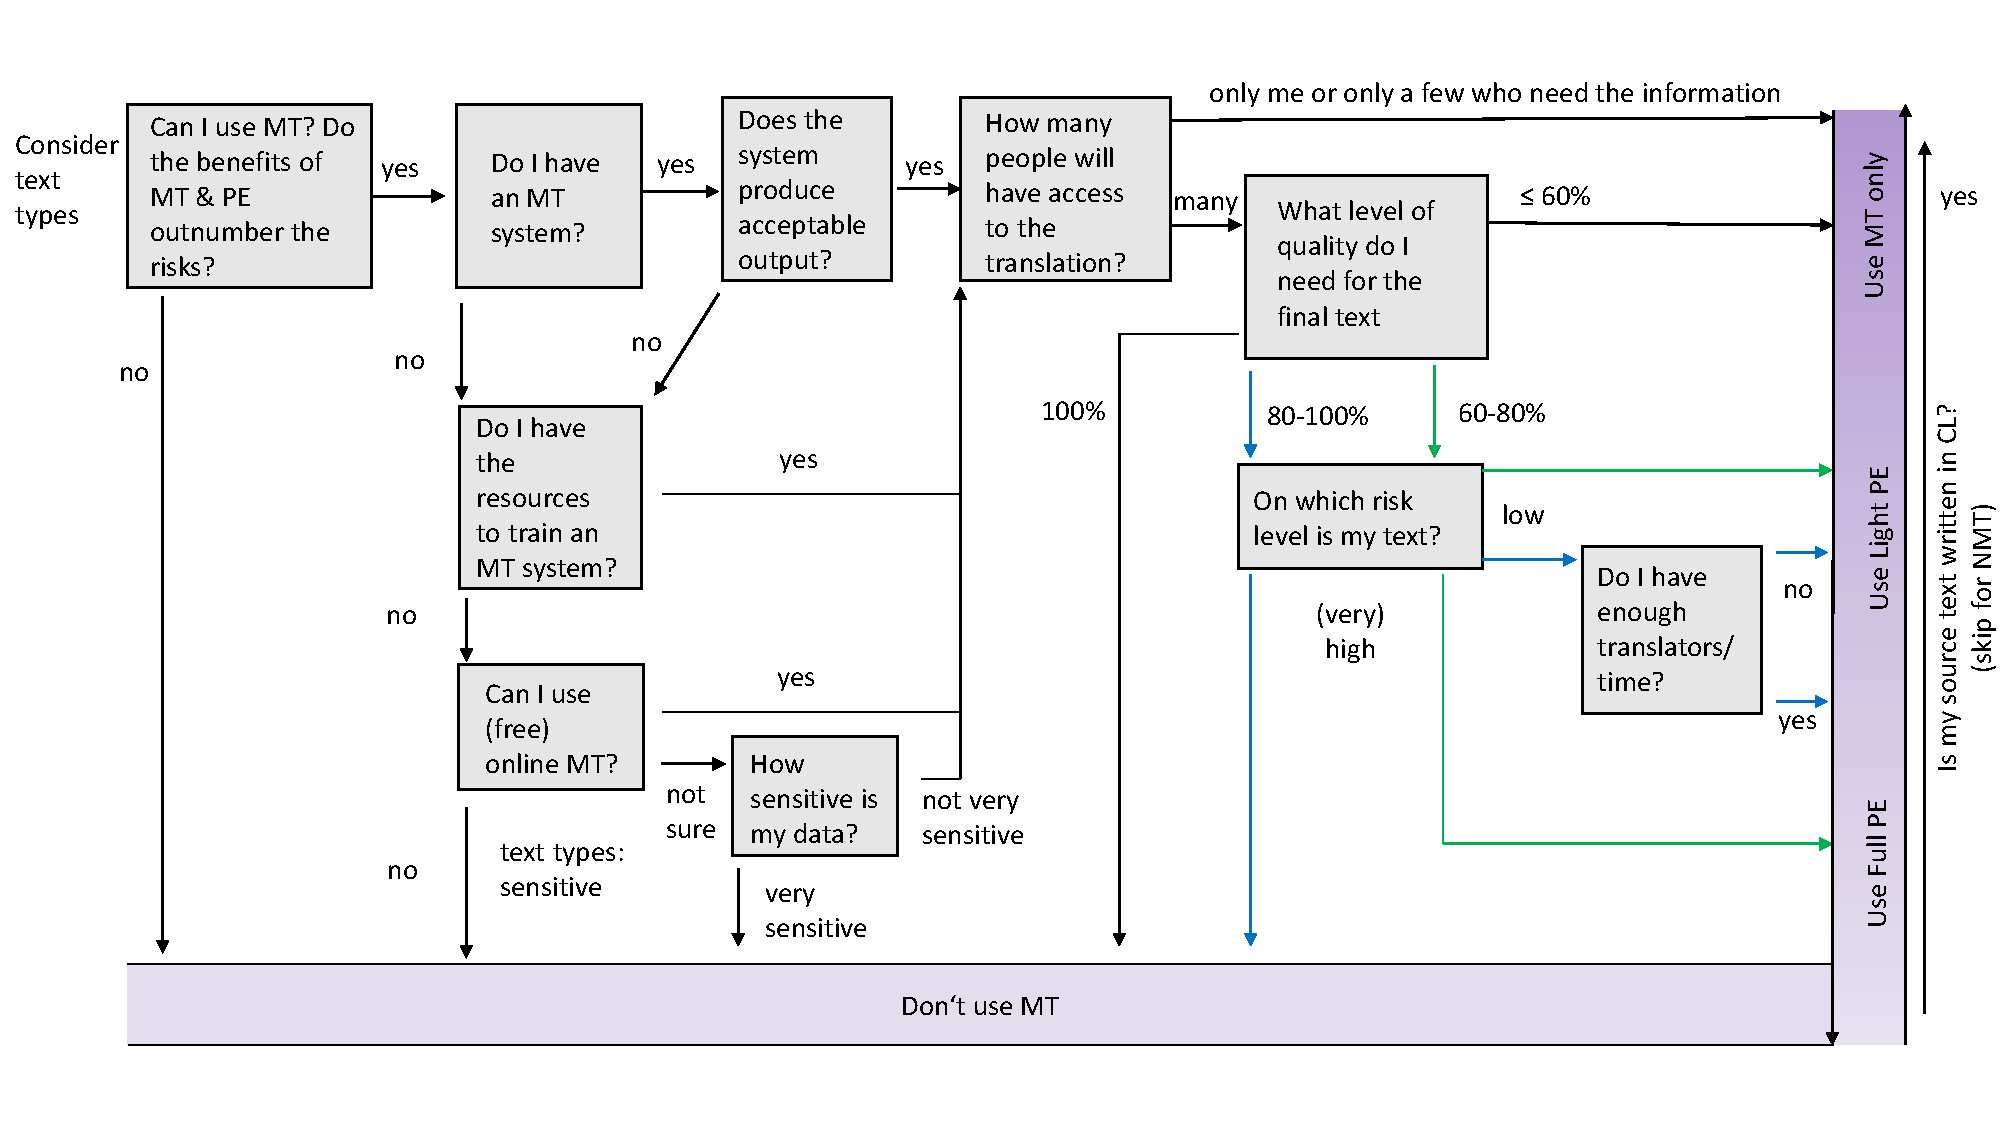
\includegraphics[width=\textwidth]{figures/art_nitzke_fig1.pdf}
\caption{Decision tree as in \citet[246]{nitzke2019risk}}
\label{fig:key:8:7}
\end{sidewaysfigure}

\citet{hor_chancen_2020} applied the decisions to the perspective of a language service pro\-vid\-er. She suggests that not all project managers should make decisions about PE projects, but only those who have PE experience. Another scenario could be that there is one (or more) designated PE expert(s). Further, she proposes to include a step for expectation management and pricing in the model -- the latter referring to the aspect that the amount of money put into the project guides the extent of the PE effort.

\newpage

\section*{Crossword puzzle -- Chapter 8}

\begin{Puzzle}{13}{14}
|{}	|{}	|{}	|{}	|{}	|{}	|{}	|{}	|{}	|{}	|[4]D	|{}	|{}	|.
|{}	|{}	|[1]P	|R	|E	|P	|A	|R	|A	|T	|I	|O	|N	|.
|{}	|{}	|{}	|{}	|{}	|{}	|{}	|{}	|{}	|{}	|S	|{}	|{}	|.
|{}	|{}	|{}	|{}	|{}	|[2]R	|{}	|{}	|{}	|{}	|T	|{}	|{}	|.
|{}	|{}	|{}	|{}	|{}	|E	|{}	|{}	|{}	|{}	|A	|{}	|{}	|.
|{}	|{}	|[5]D	|{}	|{}	|v	|{}	|{}	|{}	|{}	|N	|{}	|{}	|.
|{}	|[3]S	|E	|N	|S	|I	|T	|I	|V	|I	|T	|Y	|{}	|.
|{}	|{}	|F	|{}	|{}	|S	|{}	|{}	|{}	|{}	|{}	|{}	|{}	|.
|[7]S	|P	|E	|L	|L	|I	|N	|G	|{}	|{}	|{}	|{}	|{}	|.
|{}	|{}	|C	|{}	|{}	|O	|{}	|{}	|{}	|{}	|{}	|{}	|{}	|.
|{}	|{}	|[8]T	|U	|R	|N	|A	|R	|O	|U	|N	|D	|{}	|.
|{}	|{}	|I	|{}	|{}	|{}	|{}	|{}	|{}	|{}	|{}	|{}	|{}	|.
|{}	|{}	|V	|{}	|{}	|{}	|{}	|{}	|{}	|{}	|{}	|{}	|{}	|.
|{}	|[6]R	|E	|A	|D	|A	|B	|I	|L	|I	|T	|Y	|{}	|.
\end{Puzzle}

\begin{PuzzleClues}{\textbf{Across}}
\Clue{1}{PREPARATION}{What are the three stages of the translation process according to \cite{hofmann2012prozessgestutztes}? translation ... , translation, and translation post-processing}
\Clue{3}{SENSITIVITY}{When we assess whether a source text is appropriate for MT and PE, what are the three criteria we have to watch out for? Suitability of the source text for MT, risks, and ... of information}
\Clue{6}{READABILITY}{When a text is written in a controlled language, what is improved for the target audience?}
\Clue{7}{SPELLING}{What kind of mistakes in the source text might be corrected automatically?}
\Clue{8}{TURNAROUND}{What temporal aspect might cause very tight deadlines and might be a reason for PE, but should not still not outweigh quality considerations? ... time}
\end{PuzzleClues}

\begin{PuzzleClues}{\textbf{Down}}
\Clue{2}{REVISION}{What do we call the quality assurance step after a text has been fully post-edited or translated?}
\Clue{4}{DISTANT}{What kind of languages tend to be more difficult for MT because they are usually less linear? }
\Clue{5}{DEFECTIVE}{The source text decreases the quality of the MT output when it is very complex, very inconsistent, or ....}
\end{PuzzleClues}

\chapter{Post-editing profiles -- which competences are needed?}\label{sec:9}

    \objectives{
     You will learn...
        \begin{itemize}
            \item which competences are important for MT and PE,
            \item which job profiles might be interesting in the field of PE,
            \item what is necessary for training.
        \end{itemize}
     }


\section{PE competences}\label{sec:9:1}

Many aspects have to be considered when dealing with MT and PE. Post-editing is a complex task. Accordingly, a qualified post-editor needs specific competences to be able to fulfil all the requirements of such a task. The proposed PE competence model (\figref{fig:key:9:1}) is a further development of \citet{nitzke2019risk} based on PACTE’s (\citeyear{beeby2003building}) translation competence model and the revision competence model by \citet{robert2017towards} since they share some of the competences needed for post-editing MT output. The differences and commonalities will be explained in the following. Further, not all decisions are necessarily made by the client – some clients might need a lot of guidance when it comes to MT. A post-editor, therefore, must be able to make informed decisions concerning risk assessment as well as the integration of MT and PE in the translation workflow.

\begin{figure} 
% 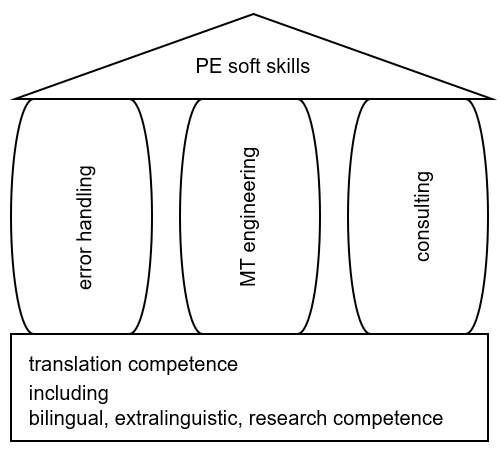
\includegraphics[height=0.3\textheight]{figures/Competence Model.PNG}
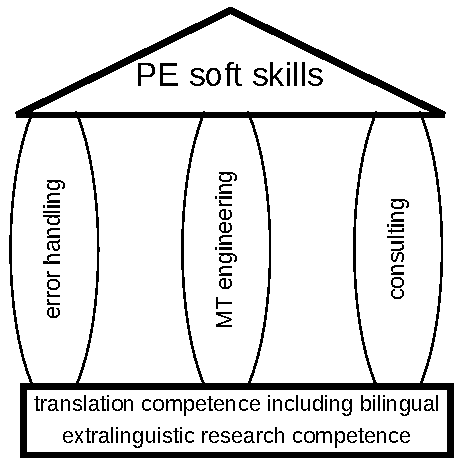
\includegraphics[height=0.3\textheight]{figures/jobprofile0.pdf}
\caption{PE competence model}
\label{fig:key:9:1}
\end{figure}

If we consider the competence model as a house of PE competences, the architecture of the house is grounded on the basic competences we also expect from professional translators: translation competences, including bilingual, extralinguistic and research competence. This is also the basis for a skilled post-editor. Translation competences have been described in different models over the years, e.g., PACTE (\citeyear{beeby2003building}), \citet{emt2009competences}, \citet{gopferich2009towards}. It is essential that post-editors are skilled translators, because they need the same basic skill set. These skills include amongst others knowledge about text type conventions, the ability to deal with style guides or controlled languages, knowledge about contrastive differences, cultural specificities, etc. As they automatically learn from data, the machines might be able to recreate some text type conventions or cultural differences, but, accordingly, the training data have to be very good and specific. Nonetheless, chances are high that the machine will make mistakes, especially in these areas. Hence, a professional translator is needed to post-edit the machine-translated output, especially when the goal is a high quality target text.

Similar to translation and revision competence, a post-editor has to have proficient knowledge of the source and target language, as monolingual PE always bears the risk that content mistakes are not recognised (see \sectref{sec:4:1:3}). This basic competence is often referred to as bilingual competence in translation competence models.

Another similarity to specialised translation and revision tasks is that a post-editor also needs to have general world knowledge as well as the relevant domain knowledge in order to properly understand the thematic subject of the source text. This knowledge can be summarised with the term extralinguistic competence. Knowledge about cultural domain differences helps the post-editor to interpret the meaning in the source text correctly and transfer it adequately to the target text.

Finally, a post-editor also needs to know where and how to find information he or she does not have, i.e. research competence is required. Depending on the thematic field of the translation, specialised (online) dictionaries might be the first choice, whereas, for others, parallel corpora or thesauri might be better options. Efficient research strategies positively influence the workflow time of a PE task. Further, the post-editor needs to learn to what extent he or she can trust the MT output, e.g. concerning the correct translation of terminology, and when MT decisions have to be changed.

\bigskip

The three pillars of the model define the additional competences: error handling, which includes error spotting, error classification, and error correction; MT engineering, which includes training and assessment of MT systems, and specialised consulting competences, which are tailored to the needs of post-editing jobs. Let us have a closer look at these competences, which will be used to describe different job profiles later in \sectref{sec:9:2}.

Let us first discuss the error-spotting competence. Different MT systems (rule-based, statistical, neural, etc.) generate different errors. Hence, it is important to know what kind of system will be used and to have knowledge of the approach used in the MT system. In recent years, neural MT has become the state-of-the-art. However, it is still plausible that statistical or hybrid systems will be used -- or that other MT approaches will be developed in the future. However, let us focus briefly on neural MT systems. Many errors generated by neural MT systems are more difficult to identify compared to statistical MT since the MT output is more fluent and seems to be correct, which leads to the problem of overlooking mistakes that are not obvious (\citealt{toral2018post}, e.g., show that pauses become fewer but longer when post-editing neural MT output). Therefore, the post-editor has to be trained to spot exactly these more fine-grained mistakes and problems. Further, the post-editor has to work efficiently and has to know which errors have to be corrected to which extent according to the respective guidelines. This means that the trained post-editor should be able to identify what kind of mistake (s)he stumbled across and whether this mistake has to be improved or not according to the job-specific guidelines in order to avoid over-corrections or over-editing (see e.g. \citealt{nitzke2020preferential} and \citealt{vardaro2019translation}). For example, different studies have shown that post-editors are primed by the MT output (e.g. \citealt{bangalore2015role}) or at least feel primed by the MT output (e.g. \citealt{moorkens2018translators}). Post-editors should be aware of these phenomena, should be able to recognise them, and should know how to deal with them. 

A post-editor needs some knowledge about machine translation engineering, although the depth of knowledge might vary across the different job profiles (see \sectref{sec:9:2}). As we have already mentioned, the different MT systems generate different problems and mistakes. Hence, a post-editor needs to know how an MT system works and which possible pitfalls it may generate. MT systems often generate other problems than human translators produce (\citealt{carl_post-editing_2015}, \citealt{nitzke2019problem}). Most of them are related to the architecture of the MT system. Knowing how MT is implemented helps to spot potential problems or difficulties. Ideally, in our view, a post-editor should be able to assess the quality of the MT training materials and even to improve the training process if necessary. Some post-editors might even help to set up a new system as they can gather and evaluate the training data.

Finally, a certain consulting competence is essential. Many clients might not be aware of the pros and cons of using machine translation systems for the translation process. Even clients that often work with translation professionals and language service providers might not be aware of risks and strategic processes as PE has only recently become established on the market. Hence, a post-editor has to inform the customer or project manager about potential risks as well as problem-solving strategies, respectively, i.e. the risk assessment should enable the post-editor to give advice on these questions, even if the post-editor is not fully responsible for the decisions regarding the overall project. A post-editor should be able to voice his/her concern if a decision seems too risky or suggest the use an MT system if it seems plausible for the job to avoid regret in hindsight. This kind of support should also be included in price calculations.   
The consulting competence goes hand in hand with risk assessment and service competences that are part of what we call PE soft skills. The risk assessment competence is very important for judging the project and supporting the client, as already discussed in \sectref{sec:7} and \sectref{sec:8}. Depending on the position of the post-editor in the whole PE process, the post-editor might be more or less responsible for the decisions concerning the use of MT. However, every post-editor should have at least little knowledge about potential risks associated with using MT systems in the PE process in order to support the clients and raise doubts if certain decisions seem risky or implausible (\citealt{kenny2020fair}).
In the field of PE, service competence means that the post-editor should be able to calculate prices competently, consciously, and transparently considering the quality of the MT output and the necessary PE effort, even though measuring and estimating PE effort is challenging (there has been a lot of research in this area, see e.g. \citealt{specia2011exploiting}; \citealt{moorkens2015correlations}; \citealt{schaeffer2014measuring}). However, it should become easier to predict the PE effort with increasing experience. Further, as the market is still developing, professional associations will be able to give more information on this topic in the future, which will facilitate a career entry. Another aspect of this competence includes handling state-of-the-art CAT and revision tools as well as integrated MT systems. The post-editor must be able to post-edit the texts efficiently according to the client’s guidelines and must be able to adapt to the client's quality expectations. Best practice would be to immediately save the post-edited or finally revised text in the TM or in the training database.

In summary, the post-editor should know the translation market, including all aspects of MT and PE, and should be able to negotiate with the customer on an equal footing. The post-editor should be able to match the needs of the customer with the set-up and conditions of the PE task as well as with the resources available to be able to make an appropriate offer that calculates a realistic time and cost frame for the job.

\bigskip

In our house of PE competence, the three pillars are framed by a roof, which represents soft skills for post-editors. As described in a similar way in the models by PACTE (\citeyear{beeby2003building}) and \citet{robert2017towards}, a PE task is also influenced by its surrounding factors such as:

\begin{itemize}
 \item psycho-physiological components, 
 \item an affinity towards the latest technological developments,
 \item the PE brief including guidelines for the PE task,
 \item the post-editor’s self-perception.
\end{itemize}{}

Some of the psycho-physiological components are especially important for post-editors, such as a well-developed ability to concentrate and sustain attention (especially in the case of repeated mistakes in the MT output), stress-resistance, logical reasoning, analytical thinking, and quick-wittedness. An affinity to working with the latest technological developments is an essential requirement to work as a post-editor, because PE tasks always go hand in hand with MT and CAT tools.

A PE job can only be accomplished successfully if the post-editor knows the target audience, the skopos of the target text, the effort that needs to go into the PE task (light vs. full PE, etc., see \sectref{sec:4}), which should all be summarised in a PE brief. Further, it has to be obvious which the post-editor's responsibilities are (e.g. maintaining of the translation memory and terminology management systems, reporting or even correcting flaws of the MT system).

\hspace*{-3pt}The broader perspective of the role and responsibilities of the post-editor should be accompanied by a new self-perception and appropriate professional ethics. When the market began to change, translators perceived PE as a mediocre task for quite a while \citep{guerberof2013professional}. However, post-editors should perceive themselves not only as mere proof-readers of MT output, but as competent language consultants and experts in creating PE processes to establish PE as a professional task in its own right. As such, they should take responsibility for the successful creation of the target text. It also requires new professional ethics that still need to be conceptualised. The new ethos should incorporate elements such as the willingness of post-editors to accept that sometimes the quality of the target text does not have to be 100\% to still fulfil the purpose of the target text, i.e. they deliver fit-for-purpose post-edited texts (\citealt{bowker2019}). In addition, post-editors (as well as revision experts) should be able to resist the urge to correct text units that do not need corrections just to prove that they are competent professionals who are indispensable to the market (cf. also \citealt{mossop2019revising} and \citealt{vardaro2019translation}).

The model we presented above shows many similarities to translation and revision models. As the basis of our PE model are general translation competences, we argue that translation and PE should not be trained separately, but PE should be added to modern translation curricula (\citealt{bernardini2020}). We recommend integrating PE in late B.A. translation programmes or even only in M.A. studies so that a general translation competence has already been developed to a certain degree. 

\section{Job profiles}\label{sec:9:2}

Our model from section \ref{sec:9:2} presents a general PE model. However, the competences we presented there can play either a major or a minor role, depending on the specialisation a post-editor wants to follow. As a consequence, the pillars in the model can vary in importance depending on the specific competences needed for the respective job profile. Let us discuss three possible job perspectives for post-editors with the help of this model. But remember that these are only suggestions and individual specialisations can be combined to different degrees.

\subsection{PE competences for post-editors}\label{sec:9:2:1}

First, we will focus on the most obvious specialisation, namely practical PE. The post-editor is actively responsible for handling the MT output in respect to the source text. The main focus is therefore error handling (\figref{fig:key:9:2:1}), which thus represents the most important pillar in our competence house. Error handling combines different sub-tasks. Post-editors must be very sensitive to error spotting and error classification, meaning that they have to be able to decide whether an error has to be corrected according to the guidelines, and of course the efficient correction of the errors. The post-editor is dependent on a well-organised PE process, including a PE brief, comprehensive PE guidelines, a well-functioning MT system, the integration into a translation memory environment, maybe a client-specific terminology database, etc. As not all clients will be familiar with the professional handling of PE tasks, it is helpful for the post-editor to have knowledge about the inner workings of MT systems for the post-editing process, e.g. for error spotting and  characterisation. In addition, it is probably helpful if they are able to consult clients, especially if they work as freelancers, but those competences have a lower priority. The risk assessment and service competences are necessary for the same reasons, but play a minor role, because they are the executing part of the PE process.

\begin{figure} 
% 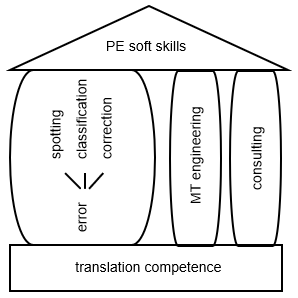
\includegraphics[height=0.4\textheight]{figures/Job Profile 1.PNG}
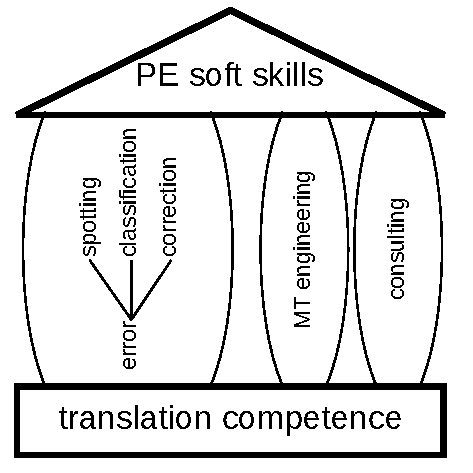
\includegraphics[height=0.4\textheight]{figures/jobprofile1.pdf}
\caption{PE competences for post-editors}
\label{fig:key:9:2:1}
\end{figure}


\subsection{PE competences for MT engineers}\label{sec:9:2:2}

A second job perspective might be called MT engineering (\figref{fig:key:9:2:2}). MT engineers are more focused on the technology. They have in-depth knowledge about how to train and maintain MT engines as well as deep knowledge of MT structures, and how to improve and evaluate the MT output. They are responsible for questions like what system is suitable for the job or for the company and what kind of data are needed for training. Further, they should have a lot of knowledge about (other) CAT tools like translation memory and terminology management systems, so that they can implement the technological support that best fits the respective project. To obtain these goals they also need basic knowledge on error handling and client consulting to be able to assess the post-editors needs and the project's requirements. Their risk assessment and service competences are an integral part of their job and can be judged as intermediate compared to the other job profiles.

\begin{figure} 
% 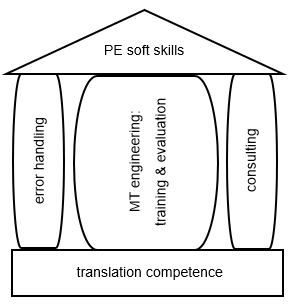
\includegraphics[height=0.4\textheight]{figures/Job Profile 2.PNG}
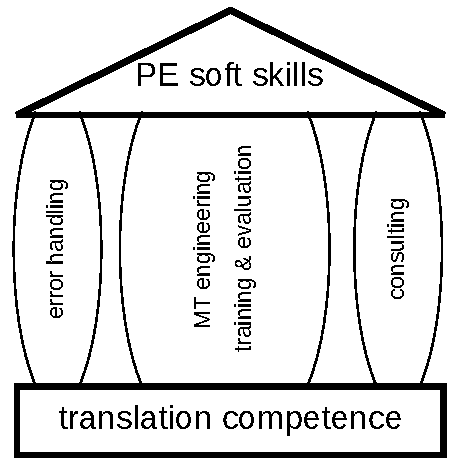
\includegraphics[height=0.4\textheight]{figures/jobprofile2.pdf}
\caption{PE competences for MT engineers}
\label{fig:key:9:2:2}
\end{figure}

\subsection{PE competences for PE consultants}\label{sec:9:2:3}

Finally, one job perspective for post-editors can be to work in a consulting position (\figref{fig:key:9:2:3}), where the main tasks are project and risk management, taking charge of the communication between the different stakeholders and making the decisions that are necessary to set up a PE project. For this, they naturally need basic knowledge on PE practice and MT engineering and they also must have profound knowledge about risk assessment and service, because they create the projects and decide which texts and projects can be post-edited and which not. They have to make decisions on the aspects we discussed in \sectref{sec:8}. Concerning the actors described in the ISO standard in section \sectref{sec:4}, PE consultants can also take the role of or work closely together with the translation service provider. 

\begin{figure} 
% 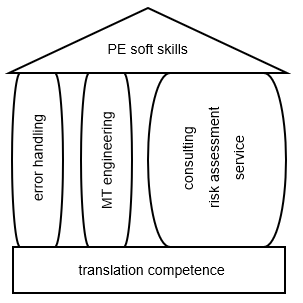
\includegraphics[height=0.4\textheight]{figures/Job Profile 3.PNG}
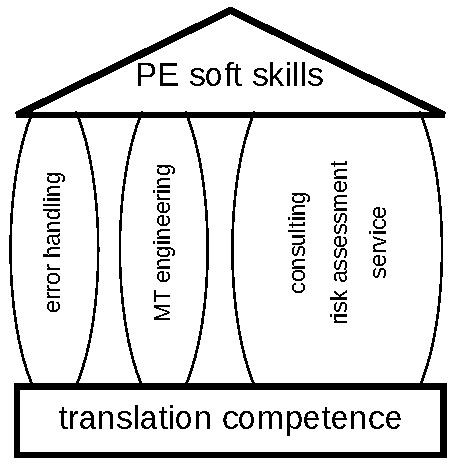
\includegraphics[height=0.4\textheight]{figures/jobprofile3.pdf}
\caption{PE competences for PE consultants}
\label{fig:key:9:2:3}
\end{figure}

\section{PE training and education}\label{sec:9:3}
\largerpage[2]
Training and education in PE should be in line with the different job profiles we described in \ref{sec:9:2}. As a prospective post-editor, you should specialise on the aspects of the job profile you are most interested in. 

If you do not have any translation experience and knowledge about translation studies at all, you should consider a translation university degree or a long term translation training to gain the relevant translation competences. When you choose a university/degree/programme, you might already keep in mind which job profile seems the most interesting for you and look at the curricula to see whether an institution offers PE courses, courses on MT or computational linguistics, and/or courses on project management.

If you are a professional translator, you have already gained a lot of PE knowledge in this book. You may want to look for courses on advanced training offered by universities or professional associations. The PE job profile is probably the closest to aim for if you want to build on your existing knowledge. Try to find a programme or some add-on courses that discuss practical aspects and offer some hands-on exercises. If you want to focus on MT engineering, you should try to gain some extra knowledge on the technology and might want to find some computer linguistic, MT, or artificial intelligence courses. If you want to focus on consulting, it would be advisable to gain some knowledge about project and risk management. Some PE practice would be helpful for the MT engineering and consulting profiles as well.

\newpage

\section*{Crossword puzzle -- chapter 9}

\begin{Puzzle}{15}{19}
|{}	|{}	|{}	|{}	|{}	|[6]P	|{}	|{}	|{}	|{}	|{}	|{}	|{}	|{}	|{}	|.
|{}	|{}	|{}	|{}	|{}	|S	|{}	|{}	|{}	|{}	|{}	|[1]T	|{}	|{}	|{}	|.
|{}	|{}	|{}	|{}	|{}	|Y	|{}	|[4]C	|{}	|{}	|{}	|R	|{}	|{}	|{}	|.
|{}	|{}	|{}	|{}	|{}	|C	|{}	|O	|{}	|{}	|{}	|A	|{}	|{}	|{}	|.
|[7]E	|R	|R	|O	|R	|H	|A	|N	|D	|L	|I	|N	|G	|{}	|{}	|.
|{}	|{}	|{}	|{}	|{}	|O	|{}	|S	|{}	|{}	|{}	|S	|{}	|{}	|{}	|.
|{}	|{}	|{}	|{}	|{}	|P	|{}	|U	|{}	|{}	|{}	|L	|{}	|{}	|{}	|.
|{}	|{}	|{}	|{}	|{}	|H	|{}	|L	|{}	|{}	|{}	|A	|{}	|{}	|{}	|.
|{}	|{}	|{}	|{}	|{}	|Y	|{}	|T	|{}	|{}	|{}	|T	|{}	|{}	|{}	|.
|{}	|{}	|{}	|{}	|{}	|S	|{}	|I	|{}	|{}	|{}	|I	|{}	|{}	|{}	|.
|{}	|{}	|{}	|{}	|{}	|I	|{}	|N	|{}	|{}	|{}	|O	|{}	|{}	|{}	|.
|{}	|{}	|{}	|{}	|{}	|O	|{}	|G	|{}	|{}	|{}	|N	|{}	|{}	|{}	|.
|{}	|{}	|{}	|{}	|{}	|L	|{}	|{}	|{}	|{}	|{}	|{}	|{}	|{}	|{}	|.
|{}	|{}	|{}	|{}	|{}	|O	|{}	|{}	|{}	|{}	|{}	|{}	|{}	|{}	|{}	|.
|{}	|{}	|{}	|[5]E	|N	|G	|I	|N	|E	|E	|R	|I	|N	|G	|{}	|.
|{}	|{}	|{}	|{}	|{}	|I	|{}	|{}	|{}	|{}	|{}	|{}	|{}	|{}	|{}	|.
|[3]C	|O	|R	|R	|E	|C	|T	|I	|O	|N	|{}	|{}	|{}	|{}	|{}	|.
|{}	|{}	|{}	|{}	|{}	|A	|{}	|{}	|{}	|{}	|{}	|{}	|{}	|{}	|{}	|.
|[2]E	|X	|T	|R	|A	|L	|I	|N	|G	|U	|I	|S	|T	|I	|C	|.
\end{Puzzle}

\begin{PuzzleClues}{\textbf{Across}}
\Clue{2}{EXTRALINGUISTIC}{What competence is needed for PE and translation from scratch that describes the knowledge about domain-specific contents, e.g. medical knowledge for translating and post-editing medical texts?}
\Clue{3}{CORRECTION}{What belongs to the error handling competence? Error spotting, error classification, and error ...}
\Clue{5}{ENGINEERING}{What do we call the competence that includes training and assessment of MT systems? MT ...}
\Clue{7}{ERRORHANDLING}{What is the most prominent competence pillar for the job profile of a post-editor?}
\end{PuzzleClues}

\begin{PuzzleClues}{\textbf{Down}}
\Clue{1}{TRANSLATION}{Which is one of the basic competences for post-editing?}
\Clue{4}{CONSULTING}{Which competence describes that post-editors must be able to inform clients about the pros and cons of using machine translation systems?}
\Clue{6}{PSYCHOPHYSIOLOGICAL}{The ability to concentrate and sustain attention, stress-resistance, logical reasoning, analytical thinking, quick-wittedness, an affinity for technologies are the ... components that are especially important for post-editors.}
\end{PuzzleClues}

\chapter{Food for thought and wrap-up}\label{sec:10}

PE has changed the field of professional translation and the market has become more diverse with more possibilities to transfer a source text into a target text. Hence, professional translators have to adapt to these changes and have to decide whether they want to broaden their range of services and offer PE. If so, many practical aspects have to be considered - many of which we could not address in this short textbook, amongst others because these aspects are often very individual. 

One example is price calculation. As in translation, there are possibly many different ways to calculate prices, e.g. per source/target text character/word/line, per hour, according to the editing distance, calculation of MT segments equally to fuzzy match segments, etc.\footnote{If you want to learn more about how to generate time or editing distance reports in memoQ, read this article \url{https://blog.memoq.com/time-tracking-and-editing-distance-reporting}, last accessed on 21 April 2021. The article is well written and might give you interesting insights even if you do not use memoQ.} Reasons for choosing one or the other are similarly manifold. Hence, it might also be reasonable to decide on  each project individually depending on the given constraints and characteristics. In the end, both translators and clients should profit from the PE process. Translators should save time (and hence gain money, not lose money) and clients should save money, as well. You can also find some more information in the \href{https://www.taus.net/academy/best-practices/postedit-best-practices/pricing-machine-translation-post-editing-guidelines}{TAUS pricing guidelines}\footnote{last accessed 11 June 2021}.


As we already briefly discussed in \sectref{sec:2}, PE has also brought interesting new aspects into the field of research, which we cannot discuss in more detail here. However, we would like to mention that both practice and research are in close dialogue with each other. \citet{arenas2014correlations}, for example, presents a study on the productivity and quality of PE in a translation memory tool compared to fuzzy and no matches. After presenting the results, she also discusses how those variables influence the pricing and that the potential benefits of PE jobs vary for each translator individually. \begin{quote}``[...] and it might be difficult to find a satisfactory solution to determine a “fair” price. In most cases, the translators should really analyze if the compensation scheme applied for a particular project is beneficial for them according to the productivity they experience during this job or series of similar jobs. Moreover, they should also consider if the use of MT and TM segments might benefit the quality they deliver, as we have seen in this study." \citet[183]{arenas2014correlations}\end{quote}
Also, different publications on PE by professional associations, e.g. \citet{ottmann_best_2017} or \citet{porsiel_machine_2017}, combine contributions of researchers and professionals.

Another aspect we only partly -- or indirectly -- focused on is machine translation ethics. Ethics is a large and important topic in artificial intelligence \citep{liao2020ethics} as with advancing AI, more and more decisions have to be made. One of the most famous ethical questions in AI is concerning self-driving cars. Although it is assumed that fewer accidents will happen when the human error is eliminated in traffic, the question remains whom to harm in an emergency situation with different actors involved \citep{bonnefon2016social}. The ethical dilemmas do not seem to be that extreme for MT systems. Nonetheless, it seems appropriate to discuss this aspect. 

So far, there has been little research on MT ethics. The main focus of the existing studies has been mainly on translating literature (e.g. \citealt{taivalkoski2019ethical} or \citealt{kenny2020machine}), which is of course not the only area that should be concerned with ethics. Some important issues are raised in \cite{moorkens2020ethics}. They discuss, for example, that the ownership of data and translations is a matter of ethical considerations as large amounts of high-quality human translations are needed to train MT systems. The use of the data is often not transparent, and it is often not clear who was asked for permission to use the data for MT training. Further, MT ethics should also be concerned with reporting the use of MT and PE giving the reader the knowledge which MT system, which PE style, and which post-editor were involved in creating the texts. This should also be true for domain-specific texts, where usually not even the translators are listed. Although most readers might not be interested in the nature of the translation, it might force the clients to fairer processes as a long list of different MT systems and post-editors, who only light post-edited the MT output might reflect badly on the client/company.

Additionally, when we talk about highlighting MT use, we might want to talk about the use of MT on websites, where the MT output is not post-edited. Let's take as an example the website of Tripadvisor\footnote{\url{https://www.tripadvisor.de/}, last accessed 10 February 2021}, where, among others, users can rate hotels, restaurants, etc. The website implements Google Translate and according to the locale settings, a translation of the users' comments is presented automatically. Under the comments there is a note in an unremarkable, gray font that the translation was created by Google and that the reader has the possibility to rate the translation. It is quite likely that many users do not see this information when they read the comment. From our perspective (taking aside all the benefits an MT systems provides on such websites), it should be open to discussion whether this report of MT use is sufficient and whether it is ethical to present it automatically.

We wanted to finish the book with this little bit of food for thought. Post-editing is still a new area and thanks to the ongoing technological developments and innovations in artificial intelligence, many changes and new challenges are still to come. Now that we are at the end of the book, think about what has changed in your perception? How do you feel about MT and PE now? You might want to go back to \sectref{sec:1} and \sectref{sec:2} and look at the answers you gave at the very beginning of this short introduction to PE. Do you still agree with your assessment or has something changed?

\newpage

\section*{Solutions to crossword puzzles}

\textbf{Section 2}

\begin{enumerate}
  \item TRANSLATOR
  \item EFFORT
  \item CATTOOLS
  \item PREEDITING
  \item RELEVANCE
  \item EMPIRICAL
  \item EYETRACKING
  \item CRITT
\end{enumerate}

\textbf{Section 3}

\begin{enumerate}
  \item WEAVER
  \item GEORGETOWN
  \item RUSSIAN
  \item ALPAC
  \item SYSTRAN
  \item WEATHERFORECASTS
  \item BABELFISH
  \item STATISTICAL
  \item INTERLINGUA
  \item NEURAL
\end{enumerate}

\textbf{Section 4}

\begin{enumerate}
    \item ENOUGH
    \item SYNTAX
    \item OUTPUT
    \item TERMINOLOGY
    \item MONOLINGUAL
    \item FULL
\end{enumerate}

\textbf{Section 5}

\begin{enumerate}
    \item CONTROLLED
    \item CREATIVITY
    \item RESTRICTIVE
    \item SUBTITLES
\end{enumerate}

\textbf{Section 6}

\begin{enumerate}
    \item SEGMENT
    \item MANAGEMENT
    \item TERMINOLOGY
    \item FUZZYMATCH
    \item EMPTY
    \item INTERACTIVE
    \item ADAPTIVE
\end{enumerate}

\textbf{Section 7}

\begin{enumerate}
    \item OPERATIVE
    \item STRATEGIC
    \item CONFIDENTIAL
    \item LIABILITY
    \item RISKS
\end{enumerate}

\textbf{Section 8}

\begin{enumerate}
    \item PREPARATION
    \item REVISION
    \item SENSITIVITY
    \item DISTANT
    \item DEFECTIVE
    \item READABILITY
    \item SPELLING
    \item TURNAROUND
\end{enumerate}

\textbf{Section 9}

\begin{enumerate}
    \item TRANSLATION
    \item EXTRALINGUISTIC
    \item CORRECTION
    \item CONSULTING
    \item ENGINEERING
    \item PSYCHOPHYSIOLOGICAL
    \item ERRORHANDLING
\end{enumerate}
 
% \include{chapters/11} 
% \include{chapters/12}
% \include{chapters/13}
% \include{chapters/14}
  
% % copy the lines above and adapt as necessary

%%%%%%%%%%%%%%%%%%%%%%%%%%%%%%%%%%%%%%%%%%%%%%%%%%%% 
%%%             Backmatter                       %%% 
%%%%%%%%%%%%%%%%%%%%%%%%%%%%%%%%%%%%%%%%%%%%%%%%%%%%

% \is{some term| see {some other term}}
\il{some language| see {some other language}}
\issa{some term with pages}{some other term also of interest}
\ilsa{some language with pages}{some other lect also of interest} 
% There is normally no need to change the backmatter section
%There is normally no need to change this file
\sloppy
\backmatter
\phantomsection%this allows hyperlink in ToC to work
{\sloppy\printbibliography[heading=references]
\cleardoublepage

\phantomsection 
\addcontentsline{toc}{chapter}{Index} 
\addcontentsline{toc}{section}{Name Index}
\ohead{\lsNameIndexTitle} 
\printindex 
\cleardoublepage
  
\phantomsection 
\addcontentsline{toc}{section}{Language Index}
\ohead{\lsLanguageIndexTitle} 
\printindex[lan] 
\cleardoublepage
  
\phantomsection 
\addcontentsline{toc}{section}{Subject Index}
\ohead{\lsSubjectIndexTitle} 
\printindex[sbj]
\ohead{} 
 
\end{document} 

% you can create your book by running
% xelatex main.tex 
